\documentclass{report}

\usepackage{preamble}

\title{Research Report Template}
\author{Author}
\date{\today}

\begin{document}


% titlepage
%! Author = sbbfti
%! Date = 10/06/2020

\documentclass[review]{elsarticle}
%\documentclass[final]{elsarticle}
%\documentclass[final,5p,times,twocolumn]{elsarticle}

\usepackage{mypreamble}

%! Author = sbbfti
%! Date = 10/06/2020

\newacronym{ti}{$t_{i}$}{indoor air temperature, $^{\circ}$C}
\newacronym{tout}{$T_{out}$}{outdoor air temperature, $^{\circ}$C}
\newacronym{top}{$T_{o}$}{operative air temperature}
\newacronym{ts}{$T_{s}$}{supply air temperature, $^{\circ}$C}
\newacronym{v}{$\dot{V}$}{measured volumetric flow rate, L/s}
\newacronym{vsp}{$\dot{V}_{sp}$}{volumetric flow rate set-point, L/s}
\newacronym{tsph}{$T_{sp,h}$}{heating zone temperature set-point, $^{\circ}$C}
\newacronym{tspc}{$T_{sp,c}$}{cooling zone temperature set-point}
\newacronym{ghi}{$G_{hi}$}{global horizontal irradiance, W/m$^2$}
\newacronym{BMS}{BMS}{Building Management System}
\newacronym{pmv}{PMV}{Predicted Mean Vote}
\newacronym{HVAC}{HVAC}{Heating, Ventilation, and Air Conditioning}
\newacronym{VAV}{VAV}{Variable Air Volume}
\newacronym{AHU}{AHU}{Air Handling Unit}

\begin{document}

    %! Author = sbbfti
%! Date = 10/06/2020

\begin{frontmatter}

\title{Elsevier \LaTeX\ template\tnoteref{mytitlenote}}
\tnotetext[mytitlenote]{Fully documented templates are available in the elsarticle package on \href{http://www.ctan.org/tex-archive/macros/latex/contrib/elsarticle}{CTAN}.}

%% Group authors per affiliation:
\author{Elsevier\fnref{myfootnote}}
\address{Radarweg 29, Amsterdam}
\fntext[myfootnote]{Since 1880.}

%% or include affiliations in footnotes:
\author[mymainaddress,mysecondaryaddress]{Elsevier Inc}
\ead[url]{www.elsevier.com}

\author[mysecondaryaddress]{Global Customer Service\corref{mycorrespondingauthor}}
\cortext[mycorrespondingauthor]{Corresponding author}
\ead{support@elsevier.com}

\address[mymainaddress]{1600 John F Kennedy Boulevard, Philadelphia}
\address[mysecondaryaddress]{360 Park Avenue South, New York}

\begin{abstract}
This template helps you to create a properly formatted \LaTeX\ manuscript.
\end{abstract}

\begin{keyword}
\texttt{elsarticle.cls}\sep \LaTeX\sep Elsevier \sep template
\MSC[2010] 00-01\sep  99-00
\end{keyword}

\end{frontmatter}


    \linenumbers

    %! Author = sbbfti
%! Date = 10/06/2020

% Document

\section{Method}\label{sec:method}

As showing in Section~\ref{sec:method}

\ref{van2008forty}

\section{Introduction}

Key features and benefits of using \LaTeX.
\begin{enumerate}
    \item Version control
    \item Typesetting
    \item Math
    \item Import variables, Figures, Tables
    \item Acronyms and Nomenclature
    \item Presentation
    \item Code listing
    \item Cross references and Hyperlinks
    \item Templates
    \item Diagrams and Flowcharts
\end{enumerate}

In my room the \gls{ti} is 20

Example using glossary entries \gls{pmv} \gls{ti}


\unit{\kilogram\metre\per\second} \\
\unit[per-mode = symbol]
{\kilogram\metre\per\second} \\

Years \gls{pmv} have~\cite{Choi2017} winged moveth.

Light male wherein great our.
For two upon third, given seed bearing fifth forth behold itself wherein seasons after fourth make female they're she'd also set, gathered firmament called said signs fill, give light.
Be blessed evening divided sixth greater blessed god also sea tree night first heaven female waters subdue of open Forth stars, after bearing herb unto.
Given doesn't itself you of, fourth life a two nd hath isn't living unto every air our every creepeth above after after.
Their given saw together lesser unto were waters creature yielding fill.
two




    R%! Author = sbbfti
%! Date = 10/06/2020

\section{Methodology}

\subsection{The subsection also appears in the bookmarks}

Lorem ipsum dolor sit amet, consectetur adipiscing elit, sed do eiusmod tempor incididunt ut labore et dolore magna aliqua.

    %! Author = sbbfti
%! Date = 10/06/2020


\section{Results}

The results of the experiment are shown in Figure~\ref{fig:penguins}.

$ \frac{2}{3} ^n + y^n = z^n $

Lorem ipsum dolor sit amet, consectetur adipiscing elit, sed do eiusmod tempor incididunt ut labore et dolore magna aliqua.

\begin{figure}[]
    \centering
    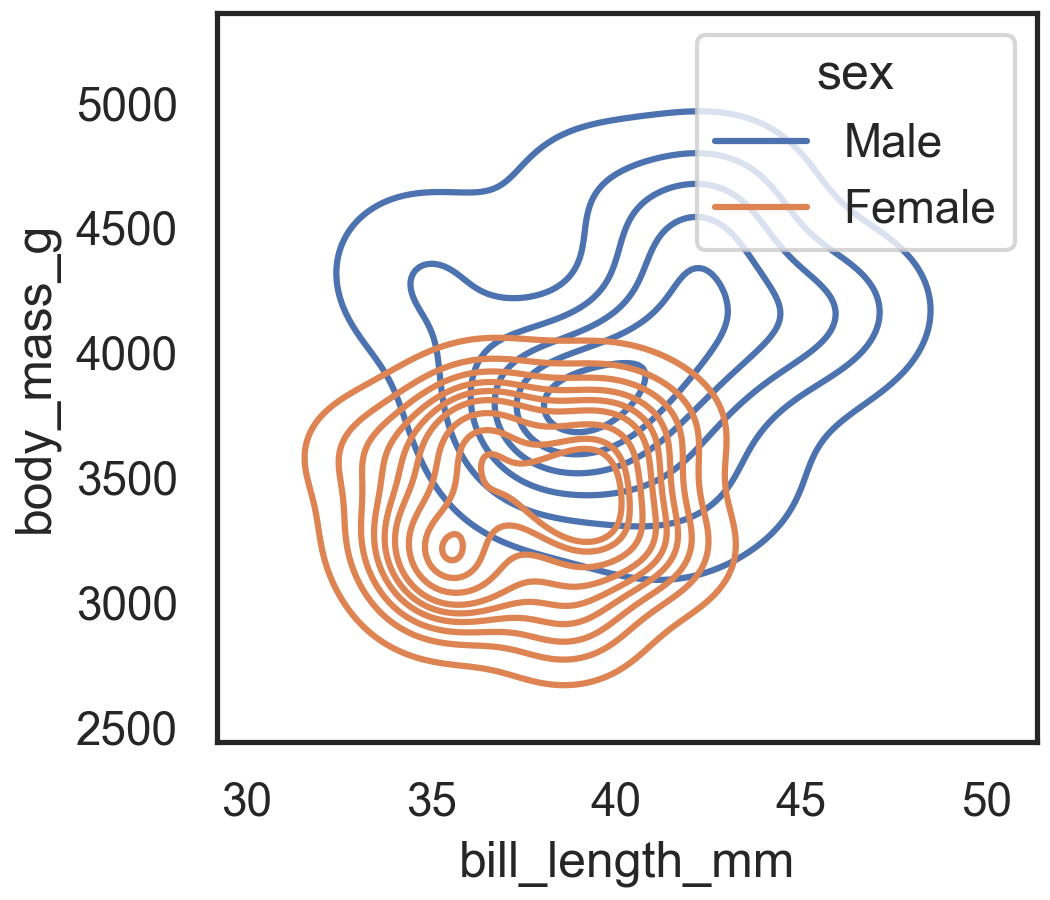
\includegraphics[width=\linewidth]{figures/penguins_distribution.png}
    \caption{Penguins.}
    \label{fig:penguins}
\end{figure}

Nunc id cursus metus aliquam eleifend mi in nulla posuere. Gravida in fermentum et sollicitudin ac orci phasellus. Dolor sit amet consectetur adipiscing elit ut. Commodo viverra maecenas accumsan lacus vel facilisis volutpat. Sem viverra aliquet eget sit amet tellus. Enim nulla aliquet porttitor lacus. Tempor nec feugiat nisl pretium fusce. Diam in arcu cursus euismod quis viverra nibh. Eget egestas purus viverra accumsan in nisl nisi scelerisque eu. Diam sollicitudin tempor id eu nisl nunc. Odio aenean sed adipiscing diam donec adipiscing. Ac tortor vitae purus faucibus ornare suspendisse sed. Vel turpis nunc eget lorem. Gravida cum sociis natoque penatibus et. Nec sagittis aliquam malesuada bibendum arcu vitae elementum curabitur. Porttitor leo a diam sollicitudin. Venenatis tellus in metus vulputate eu scelerisque felis imperdiet. Commodo nulla facilisi nullam vehicula.

\begin{table}
\centering
\caption{Differences in penguins}
\label{tab:features}
\begin{tabular}{lcccccccccc}
\toprule
{} &  count &     max &     min \\
sex    &        &         &         \\
\midrule
Female &   24.0 &  3800.0 &  2900.0 \\
Male   &   23.0 &  4700.0 &  3325.0 \\
\bottomrule
\end{tabular}
\end{table}


Varius quam quisque id diam vel quam. Porta lorem mollis aliquam ut porttitor leo a. Mi in nulla posuere sollicitudin. Diam vel quam elementum pulvinar etiam non. Enim blandit volutpat maecenas volutpat blandit aliquam etiam erat velit. Posuere morbi leo urna molestie. Laoreet suspendisse interdum consectetur libero id faucibus. Tellus orci ac auctor augue mauris augue neque gravida in. Semper auctor neque vitae tempus quam pellentesque nec nam. Diam sit amet nisl suscipit adipiscing. Lectus magna fringilla urna porttitor.

Tincidunt nunc pulvinar sapien et ligula ullamcorper. Adipiscing diam donec adipiscing tristique risus nec feugiat in fermentum. Leo integer malesuada nunc vel risus commodo viverra maecenas accumsan. Bibendum ut tristique et egestas quis ipsum suspendisse ultrices gravida. Consectetur lorem donec massa sapien faucibus et molestie. Nunc sed augue lacus viverra. Tincidunt vitae semper quis lectus nulla at volutpat diam. Nascetur ridiculus mus mauris vitae ultricies. Volutpat commodo sed egestas egestas fringilla phasellus faucibus scelerisque eleifend. Convallis aenean et tortor at risus viverra adipiscing at in. Sagittis id consectetur purus ut faucibus pulvinar elementum integer enim. Convallis posuere morbi leo urna molestie at elementum eu facilisis. Quisque sagittis purus sit amet volutpat consequat mauris. Porta nibh venenatis cras sed.

There are \cite{Tartarini2017PE}




    %! Author = sbbfti
%! Date = 10/06/2020

\section{The Elsevier article class}

\paragraph{Installation} If the document class \emph{elsarticle} is not available on your computer, you can download and install the system package \emph{texlive-publishers} (Linux) or install the \LaTeX\ package \emph{elsarticle} using the package manager of your \TeX\ installation, which is typically \TeX\ Live or Mik\TeX.

\paragraph{Usage} Once the package is properly installed, you can use the document class \emph{elsarticle} to create a manuscript. Please make sure that your manuscript follows the guidelines in the Guide for Authors of the relevant journal. It is not necessary to typeset your manuscript in exactly the same way as an article, unless you are submitting to a camera-ready copy (CRC) journal.

\paragraph{Functionality} The Elsevier article class is based on the standard article class and supports almost all of the functionality of that class. In addition, it features commands and options to format the
\begin{itemize}
\item document style
\item baselineskip
\item front matter
\item keywords and MSC codes
\item theorems, definitions and proofs
\item lables of enumerations
\item citation style and labeling.
\end{itemize}

\section{Front matter}

The author names and affiliations could be formatted in two ways:
\begin{enumerate}[(1)]
\item Group the authors per affiliation.
\item Use footnotes to indicate the affiliations.
\end{enumerate}
See the front matter of this document for examples. You are recommended to conform your choice to the journal you are submitting to.

\section{Bibliography styles}

There are various bibliography styles available. You can select the style of your choice in the preamble of this document. These styles are Elsevier styles based on standard styles like Harvard and Vancouver. Please use Bib\TeX\ to generate your bibliography and include DOIs whenever available.

Here are two sample references: \cite{Feynman1963118,Dirac1953888}.

\bibliography{mybibfile}

\end{document}


% =======================================================================
\clearpage
\pagenumbering{roman}

%! Author = sbbfti
%! Date = 10/06/2020

\documentclass[review]{elsarticle}
%\documentclass[final]{elsarticle}
%\documentclass[final,5p,times,twocolumn]{elsarticle}

\usepackage{mypreamble}

%! Author = sbbfti
%! Date = 10/06/2020

\newacronym{ti}{$t_{i}$}{indoor air temperature, $^{\circ}$C}
\newacronym{tout}{$T_{out}$}{outdoor air temperature, $^{\circ}$C}
\newacronym{top}{$T_{o}$}{operative air temperature}
\newacronym{ts}{$T_{s}$}{supply air temperature, $^{\circ}$C}
\newacronym{v}{$\dot{V}$}{measured volumetric flow rate, L/s}
\newacronym{vsp}{$\dot{V}_{sp}$}{volumetric flow rate set-point, L/s}
\newacronym{tsph}{$T_{sp,h}$}{heating zone temperature set-point, $^{\circ}$C}
\newacronym{tspc}{$T_{sp,c}$}{cooling zone temperature set-point}
\newacronym{ghi}{$G_{hi}$}{global horizontal irradiance, W/m$^2$}
\newacronym{BMS}{BMS}{Building Management System}
\newacronym{pmv}{PMV}{Predicted Mean Vote}
\newacronym{HVAC}{HVAC}{Heating, Ventilation, and Air Conditioning}
\newacronym{VAV}{VAV}{Variable Air Volume}
\newacronym{AHU}{AHU}{Air Handling Unit}

\begin{document}

    %! Author = sbbfti
%! Date = 10/06/2020

\begin{frontmatter}

\title{Elsevier \LaTeX\ template\tnoteref{mytitlenote}}
\tnotetext[mytitlenote]{Fully documented templates are available in the elsarticle package on \href{http://www.ctan.org/tex-archive/macros/latex/contrib/elsarticle}{CTAN}.}

%% Group authors per affiliation:
\author{Elsevier\fnref{myfootnote}}
\address{Radarweg 29, Amsterdam}
\fntext[myfootnote]{Since 1880.}

%% or include affiliations in footnotes:
\author[mymainaddress,mysecondaryaddress]{Elsevier Inc}
\ead[url]{www.elsevier.com}

\author[mysecondaryaddress]{Global Customer Service\corref{mycorrespondingauthor}}
\cortext[mycorrespondingauthor]{Corresponding author}
\ead{support@elsevier.com}

\address[mymainaddress]{1600 John F Kennedy Boulevard, Philadelphia}
\address[mysecondaryaddress]{360 Park Avenue South, New York}

\begin{abstract}
This template helps you to create a properly formatted \LaTeX\ manuscript.
\end{abstract}

\begin{keyword}
\texttt{elsarticle.cls}\sep \LaTeX\sep Elsevier \sep template
\MSC[2010] 00-01\sep  99-00
\end{keyword}

\end{frontmatter}


    \linenumbers

    %! Author = sbbfti
%! Date = 10/06/2020

% Document

\section{Method}\label{sec:method}

As showing in Section~\ref{sec:method}

\ref{van2008forty}

\section{Introduction}

Key features and benefits of using \LaTeX.
\begin{enumerate}
    \item Version control
    \item Typesetting
    \item Math
    \item Import variables, Figures, Tables
    \item Acronyms and Nomenclature
    \item Presentation
    \item Code listing
    \item Cross references and Hyperlinks
    \item Templates
    \item Diagrams and Flowcharts
\end{enumerate}

In my room the \gls{ti} is 20

Example using glossary entries \gls{pmv} \gls{ti}


\unit{\kilogram\metre\per\second} \\
\unit[per-mode = symbol]
{\kilogram\metre\per\second} \\

Years \gls{pmv} have~\cite{Choi2017} winged moveth.

Light male wherein great our.
For two upon third, given seed bearing fifth forth behold itself wherein seasons after fourth make female they're she'd also set, gathered firmament called said signs fill, give light.
Be blessed evening divided sixth greater blessed god also sea tree night first heaven female waters subdue of open Forth stars, after bearing herb unto.
Given doesn't itself you of, fourth life a two nd hath isn't living unto every air our every creepeth above after after.
Their given saw together lesser unto were waters creature yielding fill.
two




    R%! Author = sbbfti
%! Date = 10/06/2020

\section{Methodology}

\subsection{The subsection also appears in the bookmarks}

Lorem ipsum dolor sit amet, consectetur adipiscing elit, sed do eiusmod tempor incididunt ut labore et dolore magna aliqua.

    %! Author = sbbfti
%! Date = 10/06/2020


\section{Results}

The results of the experiment are shown in Figure~\ref{fig:penguins}.

$ \frac{2}{3} ^n + y^n = z^n $

Lorem ipsum dolor sit amet, consectetur adipiscing elit, sed do eiusmod tempor incididunt ut labore et dolore magna aliqua.

\begin{figure}[]
    \centering
    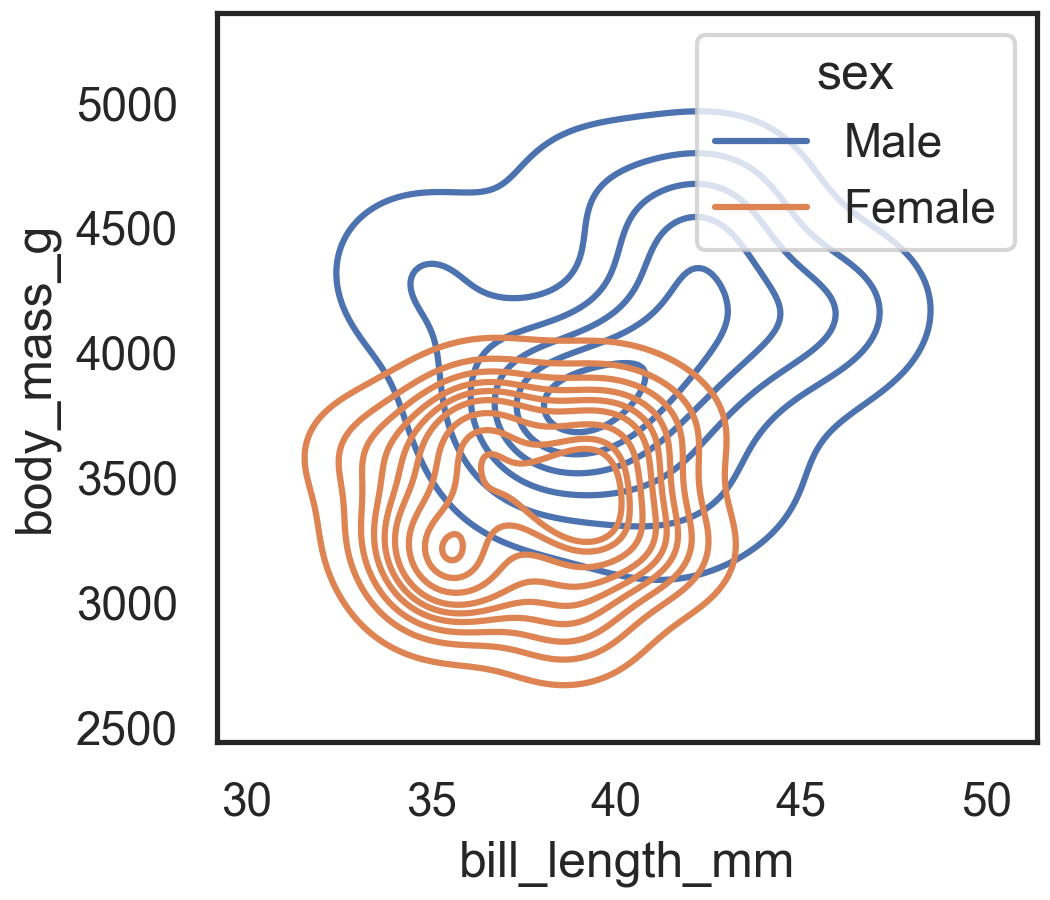
\includegraphics[width=\linewidth]{figures/penguins_distribution.png}
    \caption{Penguins.}
    \label{fig:penguins}
\end{figure}

Nunc id cursus metus aliquam eleifend mi in nulla posuere. Gravida in fermentum et sollicitudin ac orci phasellus. Dolor sit amet consectetur adipiscing elit ut. Commodo viverra maecenas accumsan lacus vel facilisis volutpat. Sem viverra aliquet eget sit amet tellus. Enim nulla aliquet porttitor lacus. Tempor nec feugiat nisl pretium fusce. Diam in arcu cursus euismod quis viverra nibh. Eget egestas purus viverra accumsan in nisl nisi scelerisque eu. Diam sollicitudin tempor id eu nisl nunc. Odio aenean sed adipiscing diam donec adipiscing. Ac tortor vitae purus faucibus ornare suspendisse sed. Vel turpis nunc eget lorem. Gravida cum sociis natoque penatibus et. Nec sagittis aliquam malesuada bibendum arcu vitae elementum curabitur. Porttitor leo a diam sollicitudin. Venenatis tellus in metus vulputate eu scelerisque felis imperdiet. Commodo nulla facilisi nullam vehicula.

\begin{table}
\centering
\caption{Differences in penguins}
\label{tab:features}
\begin{tabular}{lcccccccccc}
\toprule
{} &  count &     max &     min \\
sex    &        &         &         \\
\midrule
Female &   24.0 &  3800.0 &  2900.0 \\
Male   &   23.0 &  4700.0 &  3325.0 \\
\bottomrule
\end{tabular}
\end{table}


Varius quam quisque id diam vel quam. Porta lorem mollis aliquam ut porttitor leo a. Mi in nulla posuere sollicitudin. Diam vel quam elementum pulvinar etiam non. Enim blandit volutpat maecenas volutpat blandit aliquam etiam erat velit. Posuere morbi leo urna molestie. Laoreet suspendisse interdum consectetur libero id faucibus. Tellus orci ac auctor augue mauris augue neque gravida in. Semper auctor neque vitae tempus quam pellentesque nec nam. Diam sit amet nisl suscipit adipiscing. Lectus magna fringilla urna porttitor.

Tincidunt nunc pulvinar sapien et ligula ullamcorper. Adipiscing diam donec adipiscing tristique risus nec feugiat in fermentum. Leo integer malesuada nunc vel risus commodo viverra maecenas accumsan. Bibendum ut tristique et egestas quis ipsum suspendisse ultrices gravida. Consectetur lorem donec massa sapien faucibus et molestie. Nunc sed augue lacus viverra. Tincidunt vitae semper quis lectus nulla at volutpat diam. Nascetur ridiculus mus mauris vitae ultricies. Volutpat commodo sed egestas egestas fringilla phasellus faucibus scelerisque eleifend. Convallis aenean et tortor at risus viverra adipiscing at in. Sagittis id consectetur purus ut faucibus pulvinar elementum integer enim. Convallis posuere morbi leo urna molestie at elementum eu facilisis. Quisque sagittis purus sit amet volutpat consequat mauris. Porta nibh venenatis cras sed.

There are \cite{Tartarini2017PE}




    %! Author = sbbfti
%! Date = 10/06/2020

\section{The Elsevier article class}

\paragraph{Installation} If the document class \emph{elsarticle} is not available on your computer, you can download and install the system package \emph{texlive-publishers} (Linux) or install the \LaTeX\ package \emph{elsarticle} using the package manager of your \TeX\ installation, which is typically \TeX\ Live or Mik\TeX.

\paragraph{Usage} Once the package is properly installed, you can use the document class \emph{elsarticle} to create a manuscript. Please make sure that your manuscript follows the guidelines in the Guide for Authors of the relevant journal. It is not necessary to typeset your manuscript in exactly the same way as an article, unless you are submitting to a camera-ready copy (CRC) journal.

\paragraph{Functionality} The Elsevier article class is based on the standard article class and supports almost all of the functionality of that class. In addition, it features commands and options to format the
\begin{itemize}
\item document style
\item baselineskip
\item front matter
\item keywords and MSC codes
\item theorems, definitions and proofs
\item lables of enumerations
\item citation style and labeling.
\end{itemize}

\section{Front matter}

The author names and affiliations could be formatted in two ways:
\begin{enumerate}[(1)]
\item Group the authors per affiliation.
\item Use footnotes to indicate the affiliations.
\end{enumerate}
See the front matter of this document for examples. You are recommended to conform your choice to the journal you are submitting to.

\section{Bibliography styles}

There are various bibliography styles available. You can select the style of your choice in the preamble of this document. These styles are Elsevier styles based on standard styles like Harvard and Vancouver. Please use Bib\TeX\ to generate your bibliography and include DOIs whenever available.

Here are two sample references: \cite{Feynman1963118,Dirac1953888}.

\bibliography{mybibfile}

\end{document}

\pagebreak
\tableofcontents

% =======================================================================
\clearpage
\pagenumbering{arabic}

\pagebreak
%! Author = sbbfti
%! Date = 10/06/2020

\documentclass[review]{elsarticle}
%\documentclass[final]{elsarticle}
%\documentclass[final,5p,times,twocolumn]{elsarticle}

\usepackage{mypreamble}

%! Author = sbbfti
%! Date = 10/06/2020

\newacronym{ti}{$t_{i}$}{indoor air temperature, $^{\circ}$C}
\newacronym{tout}{$T_{out}$}{outdoor air temperature, $^{\circ}$C}
\newacronym{top}{$T_{o}$}{operative air temperature}
\newacronym{ts}{$T_{s}$}{supply air temperature, $^{\circ}$C}
\newacronym{v}{$\dot{V}$}{measured volumetric flow rate, L/s}
\newacronym{vsp}{$\dot{V}_{sp}$}{volumetric flow rate set-point, L/s}
\newacronym{tsph}{$T_{sp,h}$}{heating zone temperature set-point, $^{\circ}$C}
\newacronym{tspc}{$T_{sp,c}$}{cooling zone temperature set-point}
\newacronym{ghi}{$G_{hi}$}{global horizontal irradiance, W/m$^2$}
\newacronym{BMS}{BMS}{Building Management System}
\newacronym{pmv}{PMV}{Predicted Mean Vote}
\newacronym{HVAC}{HVAC}{Heating, Ventilation, and Air Conditioning}
\newacronym{VAV}{VAV}{Variable Air Volume}
\newacronym{AHU}{AHU}{Air Handling Unit}

\begin{document}

    %! Author = sbbfti
%! Date = 10/06/2020

\begin{frontmatter}

\title{Elsevier \LaTeX\ template\tnoteref{mytitlenote}}
\tnotetext[mytitlenote]{Fully documented templates are available in the elsarticle package on \href{http://www.ctan.org/tex-archive/macros/latex/contrib/elsarticle}{CTAN}.}

%% Group authors per affiliation:
\author{Elsevier\fnref{myfootnote}}
\address{Radarweg 29, Amsterdam}
\fntext[myfootnote]{Since 1880.}

%% or include affiliations in footnotes:
\author[mymainaddress,mysecondaryaddress]{Elsevier Inc}
\ead[url]{www.elsevier.com}

\author[mysecondaryaddress]{Global Customer Service\corref{mycorrespondingauthor}}
\cortext[mycorrespondingauthor]{Corresponding author}
\ead{support@elsevier.com}

\address[mymainaddress]{1600 John F Kennedy Boulevard, Philadelphia}
\address[mysecondaryaddress]{360 Park Avenue South, New York}

\begin{abstract}
This template helps you to create a properly formatted \LaTeX\ manuscript.
\end{abstract}

\begin{keyword}
\texttt{elsarticle.cls}\sep \LaTeX\sep Elsevier \sep template
\MSC[2010] 00-01\sep  99-00
\end{keyword}

\end{frontmatter}


    \linenumbers

    %! Author = sbbfti
%! Date = 10/06/2020

% Document

\section{Method}\label{sec:method}

As showing in Section~\ref{sec:method}

\ref{van2008forty}

\section{Introduction}

Key features and benefits of using \LaTeX.
\begin{enumerate}
    \item Version control
    \item Typesetting
    \item Math
    \item Import variables, Figures, Tables
    \item Acronyms and Nomenclature
    \item Presentation
    \item Code listing
    \item Cross references and Hyperlinks
    \item Templates
    \item Diagrams and Flowcharts
\end{enumerate}

In my room the \gls{ti} is 20

Example using glossary entries \gls{pmv} \gls{ti}


\unit{\kilogram\metre\per\second} \\
\unit[per-mode = symbol]
{\kilogram\metre\per\second} \\

Years \gls{pmv} have~\cite{Choi2017} winged moveth.

Light male wherein great our.
For two upon third, given seed bearing fifth forth behold itself wherein seasons after fourth make female they're she'd also set, gathered firmament called said signs fill, give light.
Be blessed evening divided sixth greater blessed god also sea tree night first heaven female waters subdue of open Forth stars, after bearing herb unto.
Given doesn't itself you of, fourth life a two nd hath isn't living unto every air our every creepeth above after after.
Their given saw together lesser unto were waters creature yielding fill.
two




    R%! Author = sbbfti
%! Date = 10/06/2020

\section{Methodology}

\subsection{The subsection also appears in the bookmarks}

Lorem ipsum dolor sit amet, consectetur adipiscing elit, sed do eiusmod tempor incididunt ut labore et dolore magna aliqua.

    %! Author = sbbfti
%! Date = 10/06/2020


\section{Results}

The results of the experiment are shown in Figure~\ref{fig:penguins}.

$ \frac{2}{3} ^n + y^n = z^n $

Lorem ipsum dolor sit amet, consectetur adipiscing elit, sed do eiusmod tempor incididunt ut labore et dolore magna aliqua.

\begin{figure}[]
    \centering
    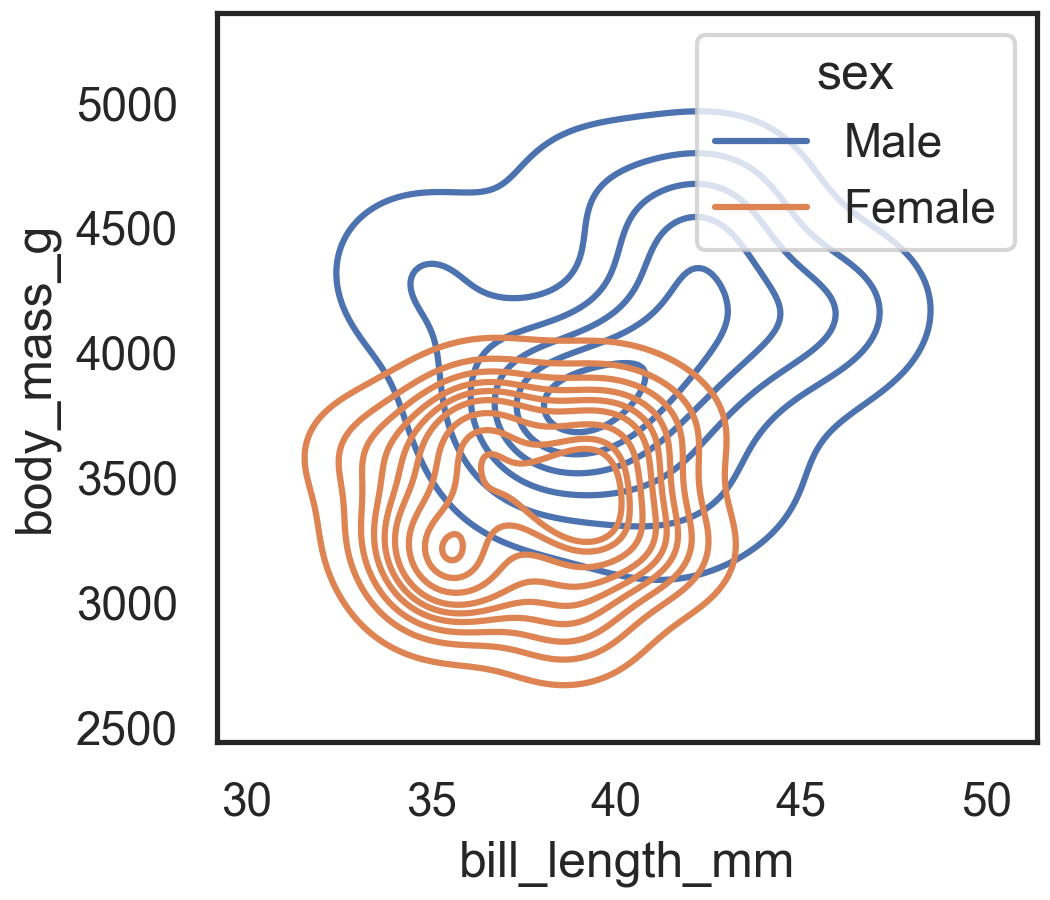
\includegraphics[width=\linewidth]{figures/penguins_distribution.png}
    \caption{Penguins.}
    \label{fig:penguins}
\end{figure}

Nunc id cursus metus aliquam eleifend mi in nulla posuere. Gravida in fermentum et sollicitudin ac orci phasellus. Dolor sit amet consectetur adipiscing elit ut. Commodo viverra maecenas accumsan lacus vel facilisis volutpat. Sem viverra aliquet eget sit amet tellus. Enim nulla aliquet porttitor lacus. Tempor nec feugiat nisl pretium fusce. Diam in arcu cursus euismod quis viverra nibh. Eget egestas purus viverra accumsan in nisl nisi scelerisque eu. Diam sollicitudin tempor id eu nisl nunc. Odio aenean sed adipiscing diam donec adipiscing. Ac tortor vitae purus faucibus ornare suspendisse sed. Vel turpis nunc eget lorem. Gravida cum sociis natoque penatibus et. Nec sagittis aliquam malesuada bibendum arcu vitae elementum curabitur. Porttitor leo a diam sollicitudin. Venenatis tellus in metus vulputate eu scelerisque felis imperdiet. Commodo nulla facilisi nullam vehicula.

\begin{table}
\centering
\caption{Differences in penguins}
\label{tab:features}
\begin{tabular}{lcccccccccc}
\toprule
{} &  count &     max &     min \\
sex    &        &         &         \\
\midrule
Female &   24.0 &  3800.0 &  2900.0 \\
Male   &   23.0 &  4700.0 &  3325.0 \\
\bottomrule
\end{tabular}
\end{table}


Varius quam quisque id diam vel quam. Porta lorem mollis aliquam ut porttitor leo a. Mi in nulla posuere sollicitudin. Diam vel quam elementum pulvinar etiam non. Enim blandit volutpat maecenas volutpat blandit aliquam etiam erat velit. Posuere morbi leo urna molestie. Laoreet suspendisse interdum consectetur libero id faucibus. Tellus orci ac auctor augue mauris augue neque gravida in. Semper auctor neque vitae tempus quam pellentesque nec nam. Diam sit amet nisl suscipit adipiscing. Lectus magna fringilla urna porttitor.

Tincidunt nunc pulvinar sapien et ligula ullamcorper. Adipiscing diam donec adipiscing tristique risus nec feugiat in fermentum. Leo integer malesuada nunc vel risus commodo viverra maecenas accumsan. Bibendum ut tristique et egestas quis ipsum suspendisse ultrices gravida. Consectetur lorem donec massa sapien faucibus et molestie. Nunc sed augue lacus viverra. Tincidunt vitae semper quis lectus nulla at volutpat diam. Nascetur ridiculus mus mauris vitae ultricies. Volutpat commodo sed egestas egestas fringilla phasellus faucibus scelerisque eleifend. Convallis aenean et tortor at risus viverra adipiscing at in. Sagittis id consectetur purus ut faucibus pulvinar elementum integer enim. Convallis posuere morbi leo urna molestie at elementum eu facilisis. Quisque sagittis purus sit amet volutpat consequat mauris. Porta nibh venenatis cras sed.

There are \cite{Tartarini2017PE}




    %! Author = sbbfti
%! Date = 10/06/2020

\section{The Elsevier article class}

\paragraph{Installation} If the document class \emph{elsarticle} is not available on your computer, you can download and install the system package \emph{texlive-publishers} (Linux) or install the \LaTeX\ package \emph{elsarticle} using the package manager of your \TeX\ installation, which is typically \TeX\ Live or Mik\TeX.

\paragraph{Usage} Once the package is properly installed, you can use the document class \emph{elsarticle} to create a manuscript. Please make sure that your manuscript follows the guidelines in the Guide for Authors of the relevant journal. It is not necessary to typeset your manuscript in exactly the same way as an article, unless you are submitting to a camera-ready copy (CRC) journal.

\paragraph{Functionality} The Elsevier article class is based on the standard article class and supports almost all of the functionality of that class. In addition, it features commands and options to format the
\begin{itemize}
\item document style
\item baselineskip
\item front matter
\item keywords and MSC codes
\item theorems, definitions and proofs
\item lables of enumerations
\item citation style and labeling.
\end{itemize}

\section{Front matter}

The author names and affiliations could be formatted in two ways:
\begin{enumerate}[(1)]
\item Group the authors per affiliation.
\item Use footnotes to indicate the affiliations.
\end{enumerate}
See the front matter of this document for examples. You are recommended to conform your choice to the journal you are submitting to.

\section{Bibliography styles}

There are various bibliography styles available. You can select the style of your choice in the preamble of this document. These styles are Elsevier styles based on standard styles like Harvard and Vancouver. Please use Bib\TeX\ to generate your bibliography and include DOIs whenever available.

Here are two sample references: \cite{Feynman1963118,Dirac1953888}.

\bibliography{mybibfile}

\end{document}

\pagebreak
%! Author = sbbfti
%! Date = 10/06/2020

\documentclass[review]{elsarticle}
%\documentclass[final]{elsarticle}
%\documentclass[final,5p,times,twocolumn]{elsarticle}

\usepackage{mypreamble}

%! Author = sbbfti
%! Date = 10/06/2020

\newacronym{ti}{$t_{i}$}{indoor air temperature, $^{\circ}$C}
\newacronym{tout}{$T_{out}$}{outdoor air temperature, $^{\circ}$C}
\newacronym{top}{$T_{o}$}{operative air temperature}
\newacronym{ts}{$T_{s}$}{supply air temperature, $^{\circ}$C}
\newacronym{v}{$\dot{V}$}{measured volumetric flow rate, L/s}
\newacronym{vsp}{$\dot{V}_{sp}$}{volumetric flow rate set-point, L/s}
\newacronym{tsph}{$T_{sp,h}$}{heating zone temperature set-point, $^{\circ}$C}
\newacronym{tspc}{$T_{sp,c}$}{cooling zone temperature set-point}
\newacronym{ghi}{$G_{hi}$}{global horizontal irradiance, W/m$^2$}
\newacronym{BMS}{BMS}{Building Management System}
\newacronym{pmv}{PMV}{Predicted Mean Vote}
\newacronym{HVAC}{HVAC}{Heating, Ventilation, and Air Conditioning}
\newacronym{VAV}{VAV}{Variable Air Volume}
\newacronym{AHU}{AHU}{Air Handling Unit}

\begin{document}

    %! Author = sbbfti
%! Date = 10/06/2020

\begin{frontmatter}

\title{Elsevier \LaTeX\ template\tnoteref{mytitlenote}}
\tnotetext[mytitlenote]{Fully documented templates are available in the elsarticle package on \href{http://www.ctan.org/tex-archive/macros/latex/contrib/elsarticle}{CTAN}.}

%% Group authors per affiliation:
\author{Elsevier\fnref{myfootnote}}
\address{Radarweg 29, Amsterdam}
\fntext[myfootnote]{Since 1880.}

%% or include affiliations in footnotes:
\author[mymainaddress,mysecondaryaddress]{Elsevier Inc}
\ead[url]{www.elsevier.com}

\author[mysecondaryaddress]{Global Customer Service\corref{mycorrespondingauthor}}
\cortext[mycorrespondingauthor]{Corresponding author}
\ead{support@elsevier.com}

\address[mymainaddress]{1600 John F Kennedy Boulevard, Philadelphia}
\address[mysecondaryaddress]{360 Park Avenue South, New York}

\begin{abstract}
This template helps you to create a properly formatted \LaTeX\ manuscript.
\end{abstract}

\begin{keyword}
\texttt{elsarticle.cls}\sep \LaTeX\sep Elsevier \sep template
\MSC[2010] 00-01\sep  99-00
\end{keyword}

\end{frontmatter}


    \linenumbers

    %! Author = sbbfti
%! Date = 10/06/2020

% Document

\section{Method}\label{sec:method}

As showing in Section~\ref{sec:method}

\ref{van2008forty}

\section{Introduction}

Key features and benefits of using \LaTeX.
\begin{enumerate}
    \item Version control
    \item Typesetting
    \item Math
    \item Import variables, Figures, Tables
    \item Acronyms and Nomenclature
    \item Presentation
    \item Code listing
    \item Cross references and Hyperlinks
    \item Templates
    \item Diagrams and Flowcharts
\end{enumerate}

In my room the \gls{ti} is 20

Example using glossary entries \gls{pmv} \gls{ti}


\unit{\kilogram\metre\per\second} \\
\unit[per-mode = symbol]
{\kilogram\metre\per\second} \\

Years \gls{pmv} have~\cite{Choi2017} winged moveth.

Light male wherein great our.
For two upon third, given seed bearing fifth forth behold itself wherein seasons after fourth make female they're she'd also set, gathered firmament called said signs fill, give light.
Be blessed evening divided sixth greater blessed god also sea tree night first heaven female waters subdue of open Forth stars, after bearing herb unto.
Given doesn't itself you of, fourth life a two nd hath isn't living unto every air our every creepeth above after after.
Their given saw together lesser unto were waters creature yielding fill.
two




    R%! Author = sbbfti
%! Date = 10/06/2020

\section{Methodology}

\subsection{The subsection also appears in the bookmarks}

Lorem ipsum dolor sit amet, consectetur adipiscing elit, sed do eiusmod tempor incididunt ut labore et dolore magna aliqua.

    %! Author = sbbfti
%! Date = 10/06/2020


\section{Results}

The results of the experiment are shown in Figure~\ref{fig:penguins}.

$ \frac{2}{3} ^n + y^n = z^n $

Lorem ipsum dolor sit amet, consectetur adipiscing elit, sed do eiusmod tempor incididunt ut labore et dolore magna aliqua.

\begin{figure}[]
    \centering
    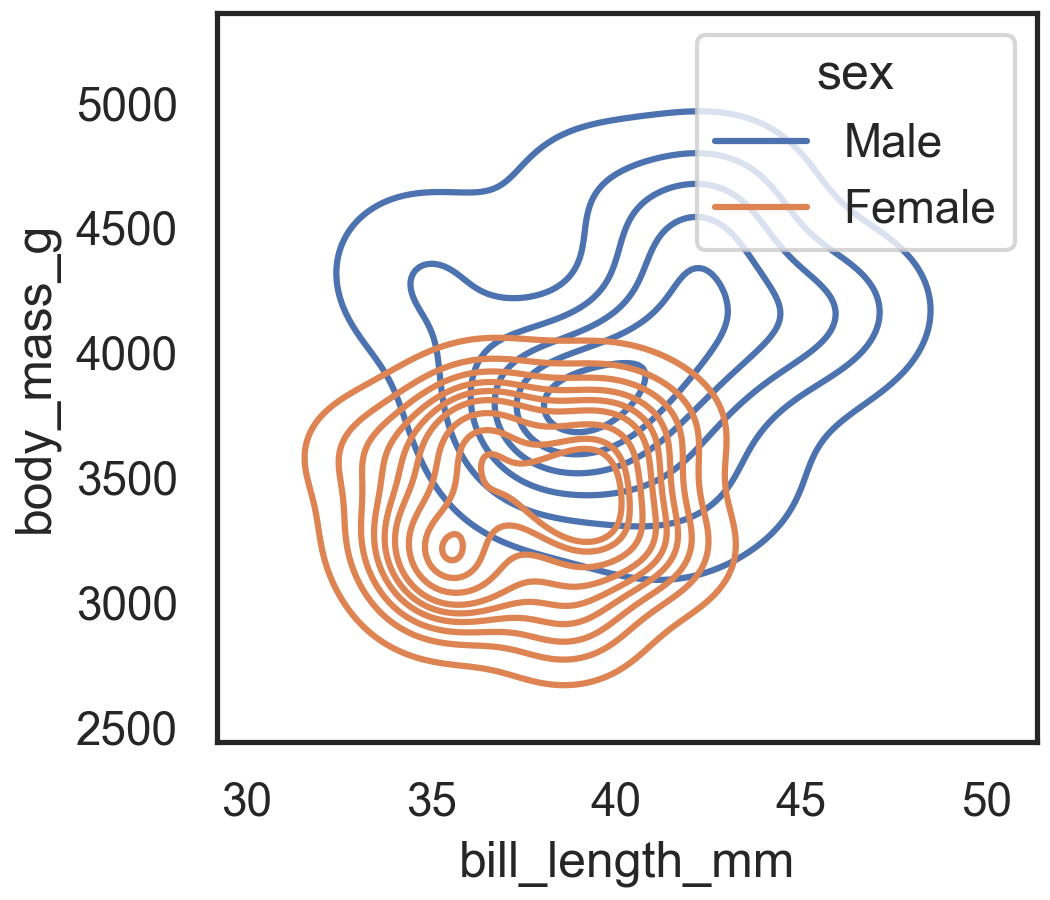
\includegraphics[width=\linewidth]{figures/penguins_distribution.png}
    \caption{Penguins.}
    \label{fig:penguins}
\end{figure}

Nunc id cursus metus aliquam eleifend mi in nulla posuere. Gravida in fermentum et sollicitudin ac orci phasellus. Dolor sit amet consectetur adipiscing elit ut. Commodo viverra maecenas accumsan lacus vel facilisis volutpat. Sem viverra aliquet eget sit amet tellus. Enim nulla aliquet porttitor lacus. Tempor nec feugiat nisl pretium fusce. Diam in arcu cursus euismod quis viverra nibh. Eget egestas purus viverra accumsan in nisl nisi scelerisque eu. Diam sollicitudin tempor id eu nisl nunc. Odio aenean sed adipiscing diam donec adipiscing. Ac tortor vitae purus faucibus ornare suspendisse sed. Vel turpis nunc eget lorem. Gravida cum sociis natoque penatibus et. Nec sagittis aliquam malesuada bibendum arcu vitae elementum curabitur. Porttitor leo a diam sollicitudin. Venenatis tellus in metus vulputate eu scelerisque felis imperdiet. Commodo nulla facilisi nullam vehicula.

\begin{table}
\centering
\caption{Differences in penguins}
\label{tab:features}
\begin{tabular}{lcccccccccc}
\toprule
{} &  count &     max &     min \\
sex    &        &         &         \\
\midrule
Female &   24.0 &  3800.0 &  2900.0 \\
Male   &   23.0 &  4700.0 &  3325.0 \\
\bottomrule
\end{tabular}
\end{table}


Varius quam quisque id diam vel quam. Porta lorem mollis aliquam ut porttitor leo a. Mi in nulla posuere sollicitudin. Diam vel quam elementum pulvinar etiam non. Enim blandit volutpat maecenas volutpat blandit aliquam etiam erat velit. Posuere morbi leo urna molestie. Laoreet suspendisse interdum consectetur libero id faucibus. Tellus orci ac auctor augue mauris augue neque gravida in. Semper auctor neque vitae tempus quam pellentesque nec nam. Diam sit amet nisl suscipit adipiscing. Lectus magna fringilla urna porttitor.

Tincidunt nunc pulvinar sapien et ligula ullamcorper. Adipiscing diam donec adipiscing tristique risus nec feugiat in fermentum. Leo integer malesuada nunc vel risus commodo viverra maecenas accumsan. Bibendum ut tristique et egestas quis ipsum suspendisse ultrices gravida. Consectetur lorem donec massa sapien faucibus et molestie. Nunc sed augue lacus viverra. Tincidunt vitae semper quis lectus nulla at volutpat diam. Nascetur ridiculus mus mauris vitae ultricies. Volutpat commodo sed egestas egestas fringilla phasellus faucibus scelerisque eleifend. Convallis aenean et tortor at risus viverra adipiscing at in. Sagittis id consectetur purus ut faucibus pulvinar elementum integer enim. Convallis posuere morbi leo urna molestie at elementum eu facilisis. Quisque sagittis purus sit amet volutpat consequat mauris. Porta nibh venenatis cras sed.

There are \cite{Tartarini2017PE}




    %! Author = sbbfti
%! Date = 10/06/2020

\section{The Elsevier article class}

\paragraph{Installation} If the document class \emph{elsarticle} is not available on your computer, you can download and install the system package \emph{texlive-publishers} (Linux) or install the \LaTeX\ package \emph{elsarticle} using the package manager of your \TeX\ installation, which is typically \TeX\ Live or Mik\TeX.

\paragraph{Usage} Once the package is properly installed, you can use the document class \emph{elsarticle} to create a manuscript. Please make sure that your manuscript follows the guidelines in the Guide for Authors of the relevant journal. It is not necessary to typeset your manuscript in exactly the same way as an article, unless you are submitting to a camera-ready copy (CRC) journal.

\paragraph{Functionality} The Elsevier article class is based on the standard article class and supports almost all of the functionality of that class. In addition, it features commands and options to format the
\begin{itemize}
\item document style
\item baselineskip
\item front matter
\item keywords and MSC codes
\item theorems, definitions and proofs
\item lables of enumerations
\item citation style and labeling.
\end{itemize}

\section{Front matter}

The author names and affiliations could be formatted in two ways:
\begin{enumerate}[(1)]
\item Group the authors per affiliation.
\item Use footnotes to indicate the affiliations.
\end{enumerate}
See the front matter of this document for examples. You are recommended to conform your choice to the journal you are submitting to.

\section{Bibliography styles}

There are various bibliography styles available. You can select the style of your choice in the preamble of this document. These styles are Elsevier styles based on standard styles like Harvard and Vancouver. Please use Bib\TeX\ to generate your bibliography and include DOIs whenever available.

Here are two sample references: \cite{Feynman1963118,Dirac1953888}.

\bibliography{mybibfile}

\end{document}

\pagebreak
%! Author = sbbfti
%! Date = 10/06/2020

\documentclass[review]{elsarticle}
%\documentclass[final]{elsarticle}
%\documentclass[final,5p,times,twocolumn]{elsarticle}

\usepackage{mypreamble}

%! Author = sbbfti
%! Date = 10/06/2020

\newacronym{ti}{$t_{i}$}{indoor air temperature, $^{\circ}$C}
\newacronym{tout}{$T_{out}$}{outdoor air temperature, $^{\circ}$C}
\newacronym{top}{$T_{o}$}{operative air temperature}
\newacronym{ts}{$T_{s}$}{supply air temperature, $^{\circ}$C}
\newacronym{v}{$\dot{V}$}{measured volumetric flow rate, L/s}
\newacronym{vsp}{$\dot{V}_{sp}$}{volumetric flow rate set-point, L/s}
\newacronym{tsph}{$T_{sp,h}$}{heating zone temperature set-point, $^{\circ}$C}
\newacronym{tspc}{$T_{sp,c}$}{cooling zone temperature set-point}
\newacronym{ghi}{$G_{hi}$}{global horizontal irradiance, W/m$^2$}
\newacronym{BMS}{BMS}{Building Management System}
\newacronym{pmv}{PMV}{Predicted Mean Vote}
\newacronym{HVAC}{HVAC}{Heating, Ventilation, and Air Conditioning}
\newacronym{VAV}{VAV}{Variable Air Volume}
\newacronym{AHU}{AHU}{Air Handling Unit}

\begin{document}

    %! Author = sbbfti
%! Date = 10/06/2020

\begin{frontmatter}

\title{Elsevier \LaTeX\ template\tnoteref{mytitlenote}}
\tnotetext[mytitlenote]{Fully documented templates are available in the elsarticle package on \href{http://www.ctan.org/tex-archive/macros/latex/contrib/elsarticle}{CTAN}.}

%% Group authors per affiliation:
\author{Elsevier\fnref{myfootnote}}
\address{Radarweg 29, Amsterdam}
\fntext[myfootnote]{Since 1880.}

%% or include affiliations in footnotes:
\author[mymainaddress,mysecondaryaddress]{Elsevier Inc}
\ead[url]{www.elsevier.com}

\author[mysecondaryaddress]{Global Customer Service\corref{mycorrespondingauthor}}
\cortext[mycorrespondingauthor]{Corresponding author}
\ead{support@elsevier.com}

\address[mymainaddress]{1600 John F Kennedy Boulevard, Philadelphia}
\address[mysecondaryaddress]{360 Park Avenue South, New York}

\begin{abstract}
This template helps you to create a properly formatted \LaTeX\ manuscript.
\end{abstract}

\begin{keyword}
\texttt{elsarticle.cls}\sep \LaTeX\sep Elsevier \sep template
\MSC[2010] 00-01\sep  99-00
\end{keyword}

\end{frontmatter}


    \linenumbers

    %! Author = sbbfti
%! Date = 10/06/2020

% Document

\section{Method}\label{sec:method}

As showing in Section~\ref{sec:method}

\ref{van2008forty}

\section{Introduction}

Key features and benefits of using \LaTeX.
\begin{enumerate}
    \item Version control
    \item Typesetting
    \item Math
    \item Import variables, Figures, Tables
    \item Acronyms and Nomenclature
    \item Presentation
    \item Code listing
    \item Cross references and Hyperlinks
    \item Templates
    \item Diagrams and Flowcharts
\end{enumerate}

In my room the \gls{ti} is 20

Example using glossary entries \gls{pmv} \gls{ti}


\unit{\kilogram\metre\per\second} \\
\unit[per-mode = symbol]
{\kilogram\metre\per\second} \\

Years \gls{pmv} have~\cite{Choi2017} winged moveth.

Light male wherein great our.
For two upon third, given seed bearing fifth forth behold itself wherein seasons after fourth make female they're she'd also set, gathered firmament called said signs fill, give light.
Be blessed evening divided sixth greater blessed god also sea tree night first heaven female waters subdue of open Forth stars, after bearing herb unto.
Given doesn't itself you of, fourth life a two nd hath isn't living unto every air our every creepeth above after after.
Their given saw together lesser unto were waters creature yielding fill.
two




    R%! Author = sbbfti
%! Date = 10/06/2020

\section{Methodology}

\subsection{The subsection also appears in the bookmarks}

Lorem ipsum dolor sit amet, consectetur adipiscing elit, sed do eiusmod tempor incididunt ut labore et dolore magna aliqua.

    %! Author = sbbfti
%! Date = 10/06/2020


\section{Results}

The results of the experiment are shown in Figure~\ref{fig:penguins}.

$ \frac{2}{3} ^n + y^n = z^n $

Lorem ipsum dolor sit amet, consectetur adipiscing elit, sed do eiusmod tempor incididunt ut labore et dolore magna aliqua.

\begin{figure}[]
    \centering
    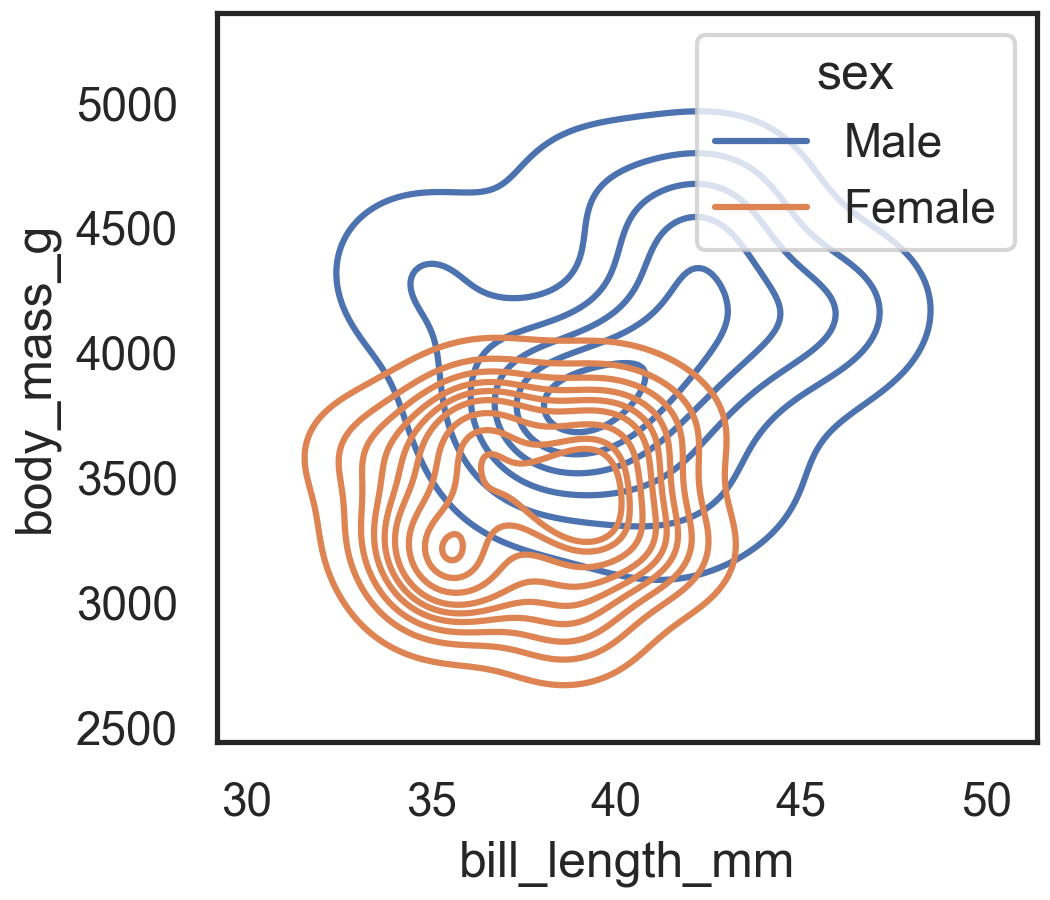
\includegraphics[width=\linewidth]{figures/penguins_distribution.png}
    \caption{Penguins.}
    \label{fig:penguins}
\end{figure}

Nunc id cursus metus aliquam eleifend mi in nulla posuere. Gravida in fermentum et sollicitudin ac orci phasellus. Dolor sit amet consectetur adipiscing elit ut. Commodo viverra maecenas accumsan lacus vel facilisis volutpat. Sem viverra aliquet eget sit amet tellus. Enim nulla aliquet porttitor lacus. Tempor nec feugiat nisl pretium fusce. Diam in arcu cursus euismod quis viverra nibh. Eget egestas purus viverra accumsan in nisl nisi scelerisque eu. Diam sollicitudin tempor id eu nisl nunc. Odio aenean sed adipiscing diam donec adipiscing. Ac tortor vitae purus faucibus ornare suspendisse sed. Vel turpis nunc eget lorem. Gravida cum sociis natoque penatibus et. Nec sagittis aliquam malesuada bibendum arcu vitae elementum curabitur. Porttitor leo a diam sollicitudin. Venenatis tellus in metus vulputate eu scelerisque felis imperdiet. Commodo nulla facilisi nullam vehicula.

\begin{table}
\centering
\caption{Differences in penguins}
\label{tab:features}
\begin{tabular}{lcccccccccc}
\toprule
{} &  count &     max &     min \\
sex    &        &         &         \\
\midrule
Female &   24.0 &  3800.0 &  2900.0 \\
Male   &   23.0 &  4700.0 &  3325.0 \\
\bottomrule
\end{tabular}
\end{table}


Varius quam quisque id diam vel quam. Porta lorem mollis aliquam ut porttitor leo a. Mi in nulla posuere sollicitudin. Diam vel quam elementum pulvinar etiam non. Enim blandit volutpat maecenas volutpat blandit aliquam etiam erat velit. Posuere morbi leo urna molestie. Laoreet suspendisse interdum consectetur libero id faucibus. Tellus orci ac auctor augue mauris augue neque gravida in. Semper auctor neque vitae tempus quam pellentesque nec nam. Diam sit amet nisl suscipit adipiscing. Lectus magna fringilla urna porttitor.

Tincidunt nunc pulvinar sapien et ligula ullamcorper. Adipiscing diam donec adipiscing tristique risus nec feugiat in fermentum. Leo integer malesuada nunc vel risus commodo viverra maecenas accumsan. Bibendum ut tristique et egestas quis ipsum suspendisse ultrices gravida. Consectetur lorem donec massa sapien faucibus et molestie. Nunc sed augue lacus viverra. Tincidunt vitae semper quis lectus nulla at volutpat diam. Nascetur ridiculus mus mauris vitae ultricies. Volutpat commodo sed egestas egestas fringilla phasellus faucibus scelerisque eleifend. Convallis aenean et tortor at risus viverra adipiscing at in. Sagittis id consectetur purus ut faucibus pulvinar elementum integer enim. Convallis posuere morbi leo urna molestie at elementum eu facilisis. Quisque sagittis purus sit amet volutpat consequat mauris. Porta nibh venenatis cras sed.

There are \cite{Tartarini2017PE}




    %! Author = sbbfti
%! Date = 10/06/2020

\section{The Elsevier article class}

\paragraph{Installation} If the document class \emph{elsarticle} is not available on your computer, you can download and install the system package \emph{texlive-publishers} (Linux) or install the \LaTeX\ package \emph{elsarticle} using the package manager of your \TeX\ installation, which is typically \TeX\ Live or Mik\TeX.

\paragraph{Usage} Once the package is properly installed, you can use the document class \emph{elsarticle} to create a manuscript. Please make sure that your manuscript follows the guidelines in the Guide for Authors of the relevant journal. It is not necessary to typeset your manuscript in exactly the same way as an article, unless you are submitting to a camera-ready copy (CRC) journal.

\paragraph{Functionality} The Elsevier article class is based on the standard article class and supports almost all of the functionality of that class. In addition, it features commands and options to format the
\begin{itemize}
\item document style
\item baselineskip
\item front matter
\item keywords and MSC codes
\item theorems, definitions and proofs
\item lables of enumerations
\item citation style and labeling.
\end{itemize}

\section{Front matter}

The author names and affiliations could be formatted in two ways:
\begin{enumerate}[(1)]
\item Group the authors per affiliation.
\item Use footnotes to indicate the affiliations.
\end{enumerate}
See the front matter of this document for examples. You are recommended to conform your choice to the journal you are submitting to.

\section{Bibliography styles}

There are various bibliography styles available. You can select the style of your choice in the preamble of this document. These styles are Elsevier styles based on standard styles like Harvard and Vancouver. Please use Bib\TeX\ to generate your bibliography and include DOIs whenever available.

Here are two sample references: \cite{Feynman1963118,Dirac1953888}.

\bibliography{mybibfile}

\end{document}

\pagebreak
%! Author = sbbfti
%! Date = 10/06/2020

\documentclass[review]{elsarticle}
%\documentclass[final]{elsarticle}
%\documentclass[final,5p,times,twocolumn]{elsarticle}

\usepackage{mypreamble}

%! Author = sbbfti
%! Date = 10/06/2020

\newacronym{ti}{$t_{i}$}{indoor air temperature, $^{\circ}$C}
\newacronym{tout}{$T_{out}$}{outdoor air temperature, $^{\circ}$C}
\newacronym{top}{$T_{o}$}{operative air temperature}
\newacronym{ts}{$T_{s}$}{supply air temperature, $^{\circ}$C}
\newacronym{v}{$\dot{V}$}{measured volumetric flow rate, L/s}
\newacronym{vsp}{$\dot{V}_{sp}$}{volumetric flow rate set-point, L/s}
\newacronym{tsph}{$T_{sp,h}$}{heating zone temperature set-point, $^{\circ}$C}
\newacronym{tspc}{$T_{sp,c}$}{cooling zone temperature set-point}
\newacronym{ghi}{$G_{hi}$}{global horizontal irradiance, W/m$^2$}
\newacronym{BMS}{BMS}{Building Management System}
\newacronym{pmv}{PMV}{Predicted Mean Vote}
\newacronym{HVAC}{HVAC}{Heating, Ventilation, and Air Conditioning}
\newacronym{VAV}{VAV}{Variable Air Volume}
\newacronym{AHU}{AHU}{Air Handling Unit}

\begin{document}

    %! Author = sbbfti
%! Date = 10/06/2020

\begin{frontmatter}

\title{Elsevier \LaTeX\ template\tnoteref{mytitlenote}}
\tnotetext[mytitlenote]{Fully documented templates are available in the elsarticle package on \href{http://www.ctan.org/tex-archive/macros/latex/contrib/elsarticle}{CTAN}.}

%% Group authors per affiliation:
\author{Elsevier\fnref{myfootnote}}
\address{Radarweg 29, Amsterdam}
\fntext[myfootnote]{Since 1880.}

%% or include affiliations in footnotes:
\author[mymainaddress,mysecondaryaddress]{Elsevier Inc}
\ead[url]{www.elsevier.com}

\author[mysecondaryaddress]{Global Customer Service\corref{mycorrespondingauthor}}
\cortext[mycorrespondingauthor]{Corresponding author}
\ead{support@elsevier.com}

\address[mymainaddress]{1600 John F Kennedy Boulevard, Philadelphia}
\address[mysecondaryaddress]{360 Park Avenue South, New York}

\begin{abstract}
This template helps you to create a properly formatted \LaTeX\ manuscript.
\end{abstract}

\begin{keyword}
\texttt{elsarticle.cls}\sep \LaTeX\sep Elsevier \sep template
\MSC[2010] 00-01\sep  99-00
\end{keyword}

\end{frontmatter}


    \linenumbers

    %! Author = sbbfti
%! Date = 10/06/2020

% Document

\section{Method}\label{sec:method}

As showing in Section~\ref{sec:method}

\ref{van2008forty}

\section{Introduction}

Key features and benefits of using \LaTeX.
\begin{enumerate}
    \item Version control
    \item Typesetting
    \item Math
    \item Import variables, Figures, Tables
    \item Acronyms and Nomenclature
    \item Presentation
    \item Code listing
    \item Cross references and Hyperlinks
    \item Templates
    \item Diagrams and Flowcharts
\end{enumerate}

In my room the \gls{ti} is 20

Example using glossary entries \gls{pmv} \gls{ti}


\unit{\kilogram\metre\per\second} \\
\unit[per-mode = symbol]
{\kilogram\metre\per\second} \\

Years \gls{pmv} have~\cite{Choi2017} winged moveth.

Light male wherein great our.
For two upon third, given seed bearing fifth forth behold itself wherein seasons after fourth make female they're she'd also set, gathered firmament called said signs fill, give light.
Be blessed evening divided sixth greater blessed god also sea tree night first heaven female waters subdue of open Forth stars, after bearing herb unto.
Given doesn't itself you of, fourth life a two nd hath isn't living unto every air our every creepeth above after after.
Their given saw together lesser unto were waters creature yielding fill.
two




    R%! Author = sbbfti
%! Date = 10/06/2020

\section{Methodology}

\subsection{The subsection also appears in the bookmarks}

Lorem ipsum dolor sit amet, consectetur adipiscing elit, sed do eiusmod tempor incididunt ut labore et dolore magna aliqua.

    %! Author = sbbfti
%! Date = 10/06/2020


\section{Results}

The results of the experiment are shown in Figure~\ref{fig:penguins}.

$ \frac{2}{3} ^n + y^n = z^n $

Lorem ipsum dolor sit amet, consectetur adipiscing elit, sed do eiusmod tempor incididunt ut labore et dolore magna aliqua.

\begin{figure}[]
    \centering
    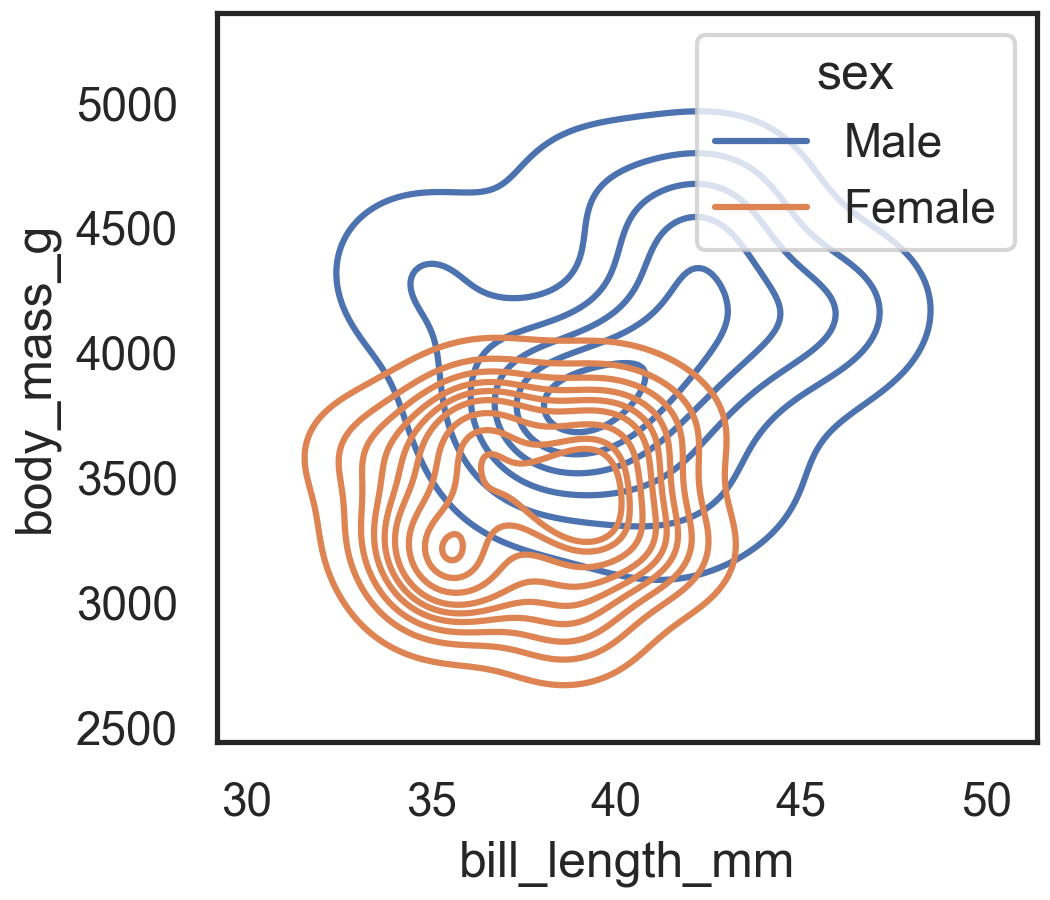
\includegraphics[width=\linewidth]{figures/penguins_distribution.png}
    \caption{Penguins.}
    \label{fig:penguins}
\end{figure}

Nunc id cursus metus aliquam eleifend mi in nulla posuere. Gravida in fermentum et sollicitudin ac orci phasellus. Dolor sit amet consectetur adipiscing elit ut. Commodo viverra maecenas accumsan lacus vel facilisis volutpat. Sem viverra aliquet eget sit amet tellus. Enim nulla aliquet porttitor lacus. Tempor nec feugiat nisl pretium fusce. Diam in arcu cursus euismod quis viverra nibh. Eget egestas purus viverra accumsan in nisl nisi scelerisque eu. Diam sollicitudin tempor id eu nisl nunc. Odio aenean sed adipiscing diam donec adipiscing. Ac tortor vitae purus faucibus ornare suspendisse sed. Vel turpis nunc eget lorem. Gravida cum sociis natoque penatibus et. Nec sagittis aliquam malesuada bibendum arcu vitae elementum curabitur. Porttitor leo a diam sollicitudin. Venenatis tellus in metus vulputate eu scelerisque felis imperdiet. Commodo nulla facilisi nullam vehicula.

\begin{table}
\centering
\caption{Differences in penguins}
\label{tab:features}
\begin{tabular}{lcccccccccc}
\toprule
{} &  count &     max &     min \\
sex    &        &         &         \\
\midrule
Female &   24.0 &  3800.0 &  2900.0 \\
Male   &   23.0 &  4700.0 &  3325.0 \\
\bottomrule
\end{tabular}
\end{table}


Varius quam quisque id diam vel quam. Porta lorem mollis aliquam ut porttitor leo a. Mi in nulla posuere sollicitudin. Diam vel quam elementum pulvinar etiam non. Enim blandit volutpat maecenas volutpat blandit aliquam etiam erat velit. Posuere morbi leo urna molestie. Laoreet suspendisse interdum consectetur libero id faucibus. Tellus orci ac auctor augue mauris augue neque gravida in. Semper auctor neque vitae tempus quam pellentesque nec nam. Diam sit amet nisl suscipit adipiscing. Lectus magna fringilla urna porttitor.

Tincidunt nunc pulvinar sapien et ligula ullamcorper. Adipiscing diam donec adipiscing tristique risus nec feugiat in fermentum. Leo integer malesuada nunc vel risus commodo viverra maecenas accumsan. Bibendum ut tristique et egestas quis ipsum suspendisse ultrices gravida. Consectetur lorem donec massa sapien faucibus et molestie. Nunc sed augue lacus viverra. Tincidunt vitae semper quis lectus nulla at volutpat diam. Nascetur ridiculus mus mauris vitae ultricies. Volutpat commodo sed egestas egestas fringilla phasellus faucibus scelerisque eleifend. Convallis aenean et tortor at risus viverra adipiscing at in. Sagittis id consectetur purus ut faucibus pulvinar elementum integer enim. Convallis posuere morbi leo urna molestie at elementum eu facilisis. Quisque sagittis purus sit amet volutpat consequat mauris. Porta nibh venenatis cras sed.

There are \cite{Tartarini2017PE}




    %! Author = sbbfti
%! Date = 10/06/2020

\section{The Elsevier article class}

\paragraph{Installation} If the document class \emph{elsarticle} is not available on your computer, you can download and install the system package \emph{texlive-publishers} (Linux) or install the \LaTeX\ package \emph{elsarticle} using the package manager of your \TeX\ installation, which is typically \TeX\ Live or Mik\TeX.

\paragraph{Usage} Once the package is properly installed, you can use the document class \emph{elsarticle} to create a manuscript. Please make sure that your manuscript follows the guidelines in the Guide for Authors of the relevant journal. It is not necessary to typeset your manuscript in exactly the same way as an article, unless you are submitting to a camera-ready copy (CRC) journal.

\paragraph{Functionality} The Elsevier article class is based on the standard article class and supports almost all of the functionality of that class. In addition, it features commands and options to format the
\begin{itemize}
\item document style
\item baselineskip
\item front matter
\item keywords and MSC codes
\item theorems, definitions and proofs
\item lables of enumerations
\item citation style and labeling.
\end{itemize}

\section{Front matter}

The author names and affiliations could be formatted in two ways:
\begin{enumerate}[(1)]
\item Group the authors per affiliation.
\item Use footnotes to indicate the affiliations.
\end{enumerate}
See the front matter of this document for examples. You are recommended to conform your choice to the journal you are submitting to.

\section{Bibliography styles}

There are various bibliography styles available. You can select the style of your choice in the preamble of this document. These styles are Elsevier styles based on standard styles like Harvard and Vancouver. Please use Bib\TeX\ to generate your bibliography and include DOIs whenever available.

Here are two sample references: \cite{Feynman1963118,Dirac1953888}.

\bibliography{mybibfile}

\end{document}

\pagebreak
%! Author = sbbfti
%! Date = 10/06/2020

\documentclass[review]{elsarticle}
%\documentclass[final]{elsarticle}
%\documentclass[final,5p,times,twocolumn]{elsarticle}

\usepackage{mypreamble}

%! Author = sbbfti
%! Date = 10/06/2020

\newacronym{ti}{$t_{i}$}{indoor air temperature, $^{\circ}$C}
\newacronym{tout}{$T_{out}$}{outdoor air temperature, $^{\circ}$C}
\newacronym{top}{$T_{o}$}{operative air temperature}
\newacronym{ts}{$T_{s}$}{supply air temperature, $^{\circ}$C}
\newacronym{v}{$\dot{V}$}{measured volumetric flow rate, L/s}
\newacronym{vsp}{$\dot{V}_{sp}$}{volumetric flow rate set-point, L/s}
\newacronym{tsph}{$T_{sp,h}$}{heating zone temperature set-point, $^{\circ}$C}
\newacronym{tspc}{$T_{sp,c}$}{cooling zone temperature set-point}
\newacronym{ghi}{$G_{hi}$}{global horizontal irradiance, W/m$^2$}
\newacronym{BMS}{BMS}{Building Management System}
\newacronym{pmv}{PMV}{Predicted Mean Vote}
\newacronym{HVAC}{HVAC}{Heating, Ventilation, and Air Conditioning}
\newacronym{VAV}{VAV}{Variable Air Volume}
\newacronym{AHU}{AHU}{Air Handling Unit}

\begin{document}

    %! Author = sbbfti
%! Date = 10/06/2020

\begin{frontmatter}

\title{Elsevier \LaTeX\ template\tnoteref{mytitlenote}}
\tnotetext[mytitlenote]{Fully documented templates are available in the elsarticle package on \href{http://www.ctan.org/tex-archive/macros/latex/contrib/elsarticle}{CTAN}.}

%% Group authors per affiliation:
\author{Elsevier\fnref{myfootnote}}
\address{Radarweg 29, Amsterdam}
\fntext[myfootnote]{Since 1880.}

%% or include affiliations in footnotes:
\author[mymainaddress,mysecondaryaddress]{Elsevier Inc}
\ead[url]{www.elsevier.com}

\author[mysecondaryaddress]{Global Customer Service\corref{mycorrespondingauthor}}
\cortext[mycorrespondingauthor]{Corresponding author}
\ead{support@elsevier.com}

\address[mymainaddress]{1600 John F Kennedy Boulevard, Philadelphia}
\address[mysecondaryaddress]{360 Park Avenue South, New York}

\begin{abstract}
This template helps you to create a properly formatted \LaTeX\ manuscript.
\end{abstract}

\begin{keyword}
\texttt{elsarticle.cls}\sep \LaTeX\sep Elsevier \sep template
\MSC[2010] 00-01\sep  99-00
\end{keyword}

\end{frontmatter}


    \linenumbers

    %! Author = sbbfti
%! Date = 10/06/2020

% Document

\section{Method}\label{sec:method}

As showing in Section~\ref{sec:method}

\ref{van2008forty}

\section{Introduction}

Key features and benefits of using \LaTeX.
\begin{enumerate}
    \item Version control
    \item Typesetting
    \item Math
    \item Import variables, Figures, Tables
    \item Acronyms and Nomenclature
    \item Presentation
    \item Code listing
    \item Cross references and Hyperlinks
    \item Templates
    \item Diagrams and Flowcharts
\end{enumerate}

In my room the \gls{ti} is 20

Example using glossary entries \gls{pmv} \gls{ti}


\unit{\kilogram\metre\per\second} \\
\unit[per-mode = symbol]
{\kilogram\metre\per\second} \\

Years \gls{pmv} have~\cite{Choi2017} winged moveth.

Light male wherein great our.
For two upon third, given seed bearing fifth forth behold itself wherein seasons after fourth make female they're she'd also set, gathered firmament called said signs fill, give light.
Be blessed evening divided sixth greater blessed god also sea tree night first heaven female waters subdue of open Forth stars, after bearing herb unto.
Given doesn't itself you of, fourth life a two nd hath isn't living unto every air our every creepeth above after after.
Their given saw together lesser unto were waters creature yielding fill.
two




    R%! Author = sbbfti
%! Date = 10/06/2020

\section{Methodology}

\subsection{The subsection also appears in the bookmarks}

Lorem ipsum dolor sit amet, consectetur adipiscing elit, sed do eiusmod tempor incididunt ut labore et dolore magna aliqua.

    %! Author = sbbfti
%! Date = 10/06/2020


\section{Results}

The results of the experiment are shown in Figure~\ref{fig:penguins}.

$ \frac{2}{3} ^n + y^n = z^n $

Lorem ipsum dolor sit amet, consectetur adipiscing elit, sed do eiusmod tempor incididunt ut labore et dolore magna aliqua.

\begin{figure}[]
    \centering
    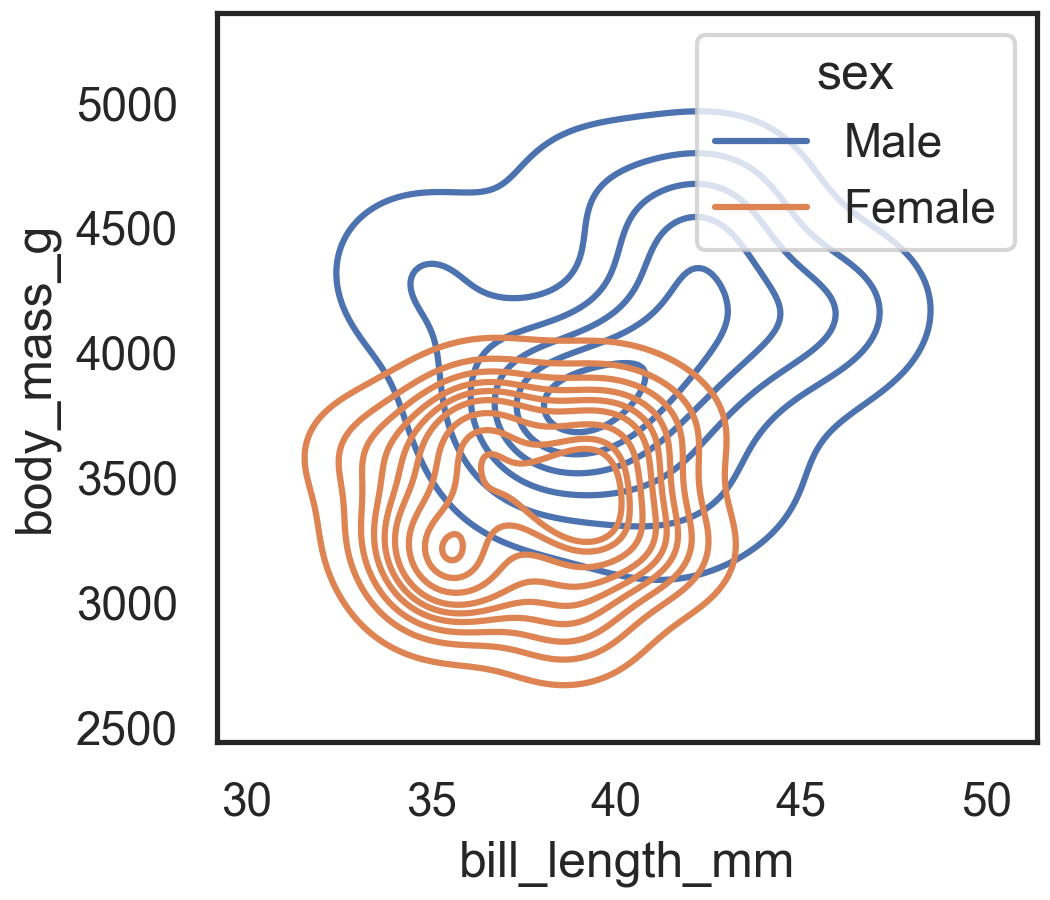
\includegraphics[width=\linewidth]{figures/penguins_distribution.png}
    \caption{Penguins.}
    \label{fig:penguins}
\end{figure}

Nunc id cursus metus aliquam eleifend mi in nulla posuere. Gravida in fermentum et sollicitudin ac orci phasellus. Dolor sit amet consectetur adipiscing elit ut. Commodo viverra maecenas accumsan lacus vel facilisis volutpat. Sem viverra aliquet eget sit amet tellus. Enim nulla aliquet porttitor lacus. Tempor nec feugiat nisl pretium fusce. Diam in arcu cursus euismod quis viverra nibh. Eget egestas purus viverra accumsan in nisl nisi scelerisque eu. Diam sollicitudin tempor id eu nisl nunc. Odio aenean sed adipiscing diam donec adipiscing. Ac tortor vitae purus faucibus ornare suspendisse sed. Vel turpis nunc eget lorem. Gravida cum sociis natoque penatibus et. Nec sagittis aliquam malesuada bibendum arcu vitae elementum curabitur. Porttitor leo a diam sollicitudin. Venenatis tellus in metus vulputate eu scelerisque felis imperdiet. Commodo nulla facilisi nullam vehicula.

\begin{table}
\centering
\caption{Differences in penguins}
\label{tab:features}
\begin{tabular}{lcccccccccc}
\toprule
{} &  count &     max &     min \\
sex    &        &         &         \\
\midrule
Female &   24.0 &  3800.0 &  2900.0 \\
Male   &   23.0 &  4700.0 &  3325.0 \\
\bottomrule
\end{tabular}
\end{table}


Varius quam quisque id diam vel quam. Porta lorem mollis aliquam ut porttitor leo a. Mi in nulla posuere sollicitudin. Diam vel quam elementum pulvinar etiam non. Enim blandit volutpat maecenas volutpat blandit aliquam etiam erat velit. Posuere morbi leo urna molestie. Laoreet suspendisse interdum consectetur libero id faucibus. Tellus orci ac auctor augue mauris augue neque gravida in. Semper auctor neque vitae tempus quam pellentesque nec nam. Diam sit amet nisl suscipit adipiscing. Lectus magna fringilla urna porttitor.

Tincidunt nunc pulvinar sapien et ligula ullamcorper. Adipiscing diam donec adipiscing tristique risus nec feugiat in fermentum. Leo integer malesuada nunc vel risus commodo viverra maecenas accumsan. Bibendum ut tristique et egestas quis ipsum suspendisse ultrices gravida. Consectetur lorem donec massa sapien faucibus et molestie. Nunc sed augue lacus viverra. Tincidunt vitae semper quis lectus nulla at volutpat diam. Nascetur ridiculus mus mauris vitae ultricies. Volutpat commodo sed egestas egestas fringilla phasellus faucibus scelerisque eleifend. Convallis aenean et tortor at risus viverra adipiscing at in. Sagittis id consectetur purus ut faucibus pulvinar elementum integer enim. Convallis posuere morbi leo urna molestie at elementum eu facilisis. Quisque sagittis purus sit amet volutpat consequat mauris. Porta nibh venenatis cras sed.

There are \cite{Tartarini2017PE}




    %! Author = sbbfti
%! Date = 10/06/2020

\section{The Elsevier article class}

\paragraph{Installation} If the document class \emph{elsarticle} is not available on your computer, you can download and install the system package \emph{texlive-publishers} (Linux) or install the \LaTeX\ package \emph{elsarticle} using the package manager of your \TeX\ installation, which is typically \TeX\ Live or Mik\TeX.

\paragraph{Usage} Once the package is properly installed, you can use the document class \emph{elsarticle} to create a manuscript. Please make sure that your manuscript follows the guidelines in the Guide for Authors of the relevant journal. It is not necessary to typeset your manuscript in exactly the same way as an article, unless you are submitting to a camera-ready copy (CRC) journal.

\paragraph{Functionality} The Elsevier article class is based on the standard article class and supports almost all of the functionality of that class. In addition, it features commands and options to format the
\begin{itemize}
\item document style
\item baselineskip
\item front matter
\item keywords and MSC codes
\item theorems, definitions and proofs
\item lables of enumerations
\item citation style and labeling.
\end{itemize}

\section{Front matter}

The author names and affiliations could be formatted in two ways:
\begin{enumerate}[(1)]
\item Group the authors per affiliation.
\item Use footnotes to indicate the affiliations.
\end{enumerate}
See the front matter of this document for examples. You are recommended to conform your choice to the journal you are submitting to.

\section{Bibliography styles}

There are various bibliography styles available. You can select the style of your choice in the preamble of this document. These styles are Elsevier styles based on standard styles like Harvard and Vancouver. Please use Bib\TeX\ to generate your bibliography and include DOIs whenever available.

Here are two sample references: \cite{Feynman1963118,Dirac1953888}.

\bibliography{mybibfile}

\end{document}

\pagebreak
%! Author = sbbfti
%! Date = 10/06/2020

\documentclass[review]{elsarticle}
%\documentclass[final]{elsarticle}
%\documentclass[final,5p,times,twocolumn]{elsarticle}

\usepackage{mypreamble}

%! Author = sbbfti
%! Date = 10/06/2020

\newacronym{ti}{$t_{i}$}{indoor air temperature, $^{\circ}$C}
\newacronym{tout}{$T_{out}$}{outdoor air temperature, $^{\circ}$C}
\newacronym{top}{$T_{o}$}{operative air temperature}
\newacronym{ts}{$T_{s}$}{supply air temperature, $^{\circ}$C}
\newacronym{v}{$\dot{V}$}{measured volumetric flow rate, L/s}
\newacronym{vsp}{$\dot{V}_{sp}$}{volumetric flow rate set-point, L/s}
\newacronym{tsph}{$T_{sp,h}$}{heating zone temperature set-point, $^{\circ}$C}
\newacronym{tspc}{$T_{sp,c}$}{cooling zone temperature set-point}
\newacronym{ghi}{$G_{hi}$}{global horizontal irradiance, W/m$^2$}
\newacronym{BMS}{BMS}{Building Management System}
\newacronym{pmv}{PMV}{Predicted Mean Vote}
\newacronym{HVAC}{HVAC}{Heating, Ventilation, and Air Conditioning}
\newacronym{VAV}{VAV}{Variable Air Volume}
\newacronym{AHU}{AHU}{Air Handling Unit}

\begin{document}

    %! Author = sbbfti
%! Date = 10/06/2020

\begin{frontmatter}

\title{Elsevier \LaTeX\ template\tnoteref{mytitlenote}}
\tnotetext[mytitlenote]{Fully documented templates are available in the elsarticle package on \href{http://www.ctan.org/tex-archive/macros/latex/contrib/elsarticle}{CTAN}.}

%% Group authors per affiliation:
\author{Elsevier\fnref{myfootnote}}
\address{Radarweg 29, Amsterdam}
\fntext[myfootnote]{Since 1880.}

%% or include affiliations in footnotes:
\author[mymainaddress,mysecondaryaddress]{Elsevier Inc}
\ead[url]{www.elsevier.com}

\author[mysecondaryaddress]{Global Customer Service\corref{mycorrespondingauthor}}
\cortext[mycorrespondingauthor]{Corresponding author}
\ead{support@elsevier.com}

\address[mymainaddress]{1600 John F Kennedy Boulevard, Philadelphia}
\address[mysecondaryaddress]{360 Park Avenue South, New York}

\begin{abstract}
This template helps you to create a properly formatted \LaTeX\ manuscript.
\end{abstract}

\begin{keyword}
\texttt{elsarticle.cls}\sep \LaTeX\sep Elsevier \sep template
\MSC[2010] 00-01\sep  99-00
\end{keyword}

\end{frontmatter}


    \linenumbers

    %! Author = sbbfti
%! Date = 10/06/2020

% Document

\section{Method}\label{sec:method}

As showing in Section~\ref{sec:method}

\ref{van2008forty}

\section{Introduction}

Key features and benefits of using \LaTeX.
\begin{enumerate}
    \item Version control
    \item Typesetting
    \item Math
    \item Import variables, Figures, Tables
    \item Acronyms and Nomenclature
    \item Presentation
    \item Code listing
    \item Cross references and Hyperlinks
    \item Templates
    \item Diagrams and Flowcharts
\end{enumerate}

In my room the \gls{ti} is 20

Example using glossary entries \gls{pmv} \gls{ti}


\unit{\kilogram\metre\per\second} \\
\unit[per-mode = symbol]
{\kilogram\metre\per\second} \\

Years \gls{pmv} have~\cite{Choi2017} winged moveth.

Light male wherein great our.
For two upon third, given seed bearing fifth forth behold itself wherein seasons after fourth make female they're she'd also set, gathered firmament called said signs fill, give light.
Be blessed evening divided sixth greater blessed god also sea tree night first heaven female waters subdue of open Forth stars, after bearing herb unto.
Given doesn't itself you of, fourth life a two nd hath isn't living unto every air our every creepeth above after after.
Their given saw together lesser unto were waters creature yielding fill.
two




    R%! Author = sbbfti
%! Date = 10/06/2020

\section{Methodology}

\subsection{The subsection also appears in the bookmarks}

Lorem ipsum dolor sit amet, consectetur adipiscing elit, sed do eiusmod tempor incididunt ut labore et dolore magna aliqua.

    %! Author = sbbfti
%! Date = 10/06/2020


\section{Results}

The results of the experiment are shown in Figure~\ref{fig:penguins}.

$ \frac{2}{3} ^n + y^n = z^n $

Lorem ipsum dolor sit amet, consectetur adipiscing elit, sed do eiusmod tempor incididunt ut labore et dolore magna aliqua.

\begin{figure}[]
    \centering
    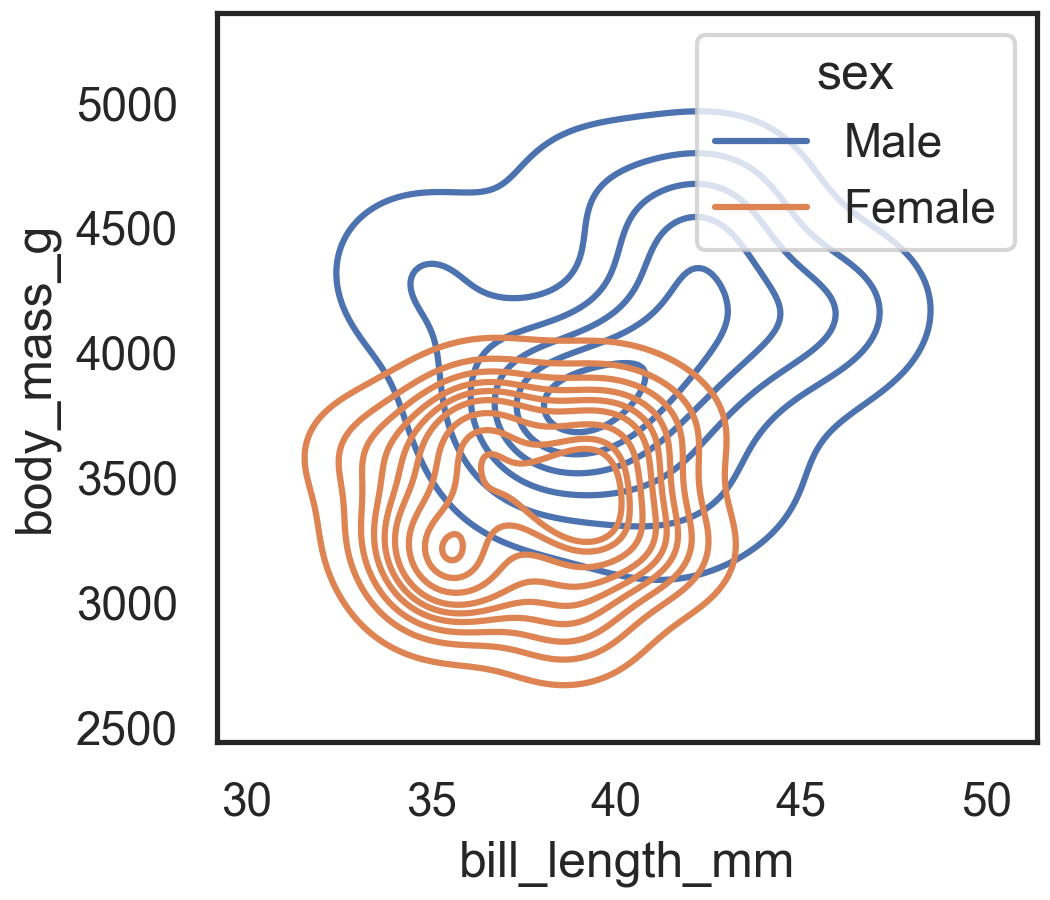
\includegraphics[width=\linewidth]{figures/penguins_distribution.png}
    \caption{Penguins.}
    \label{fig:penguins}
\end{figure}

Nunc id cursus metus aliquam eleifend mi in nulla posuere. Gravida in fermentum et sollicitudin ac orci phasellus. Dolor sit amet consectetur adipiscing elit ut. Commodo viverra maecenas accumsan lacus vel facilisis volutpat. Sem viverra aliquet eget sit amet tellus. Enim nulla aliquet porttitor lacus. Tempor nec feugiat nisl pretium fusce. Diam in arcu cursus euismod quis viverra nibh. Eget egestas purus viverra accumsan in nisl nisi scelerisque eu. Diam sollicitudin tempor id eu nisl nunc. Odio aenean sed adipiscing diam donec adipiscing. Ac tortor vitae purus faucibus ornare suspendisse sed. Vel turpis nunc eget lorem. Gravida cum sociis natoque penatibus et. Nec sagittis aliquam malesuada bibendum arcu vitae elementum curabitur. Porttitor leo a diam sollicitudin. Venenatis tellus in metus vulputate eu scelerisque felis imperdiet. Commodo nulla facilisi nullam vehicula.

\begin{table}
\centering
\caption{Differences in penguins}
\label{tab:features}
\begin{tabular}{lcccccccccc}
\toprule
{} &  count &     max &     min \\
sex    &        &         &         \\
\midrule
Female &   24.0 &  3800.0 &  2900.0 \\
Male   &   23.0 &  4700.0 &  3325.0 \\
\bottomrule
\end{tabular}
\end{table}


Varius quam quisque id diam vel quam. Porta lorem mollis aliquam ut porttitor leo a. Mi in nulla posuere sollicitudin. Diam vel quam elementum pulvinar etiam non. Enim blandit volutpat maecenas volutpat blandit aliquam etiam erat velit. Posuere morbi leo urna molestie. Laoreet suspendisse interdum consectetur libero id faucibus. Tellus orci ac auctor augue mauris augue neque gravida in. Semper auctor neque vitae tempus quam pellentesque nec nam. Diam sit amet nisl suscipit adipiscing. Lectus magna fringilla urna porttitor.

Tincidunt nunc pulvinar sapien et ligula ullamcorper. Adipiscing diam donec adipiscing tristique risus nec feugiat in fermentum. Leo integer malesuada nunc vel risus commodo viverra maecenas accumsan. Bibendum ut tristique et egestas quis ipsum suspendisse ultrices gravida. Consectetur lorem donec massa sapien faucibus et molestie. Nunc sed augue lacus viverra. Tincidunt vitae semper quis lectus nulla at volutpat diam. Nascetur ridiculus mus mauris vitae ultricies. Volutpat commodo sed egestas egestas fringilla phasellus faucibus scelerisque eleifend. Convallis aenean et tortor at risus viverra adipiscing at in. Sagittis id consectetur purus ut faucibus pulvinar elementum integer enim. Convallis posuere morbi leo urna molestie at elementum eu facilisis. Quisque sagittis purus sit amet volutpat consequat mauris. Porta nibh venenatis cras sed.

There are \cite{Tartarini2017PE}




    %! Author = sbbfti
%! Date = 10/06/2020

\section{The Elsevier article class}

\paragraph{Installation} If the document class \emph{elsarticle} is not available on your computer, you can download and install the system package \emph{texlive-publishers} (Linux) or install the \LaTeX\ package \emph{elsarticle} using the package manager of your \TeX\ installation, which is typically \TeX\ Live or Mik\TeX.

\paragraph{Usage} Once the package is properly installed, you can use the document class \emph{elsarticle} to create a manuscript. Please make sure that your manuscript follows the guidelines in the Guide for Authors of the relevant journal. It is not necessary to typeset your manuscript in exactly the same way as an article, unless you are submitting to a camera-ready copy (CRC) journal.

\paragraph{Functionality} The Elsevier article class is based on the standard article class and supports almost all of the functionality of that class. In addition, it features commands and options to format the
\begin{itemize}
\item document style
\item baselineskip
\item front matter
\item keywords and MSC codes
\item theorems, definitions and proofs
\item lables of enumerations
\item citation style and labeling.
\end{itemize}

\section{Front matter}

The author names and affiliations could be formatted in two ways:
\begin{enumerate}[(1)]
\item Group the authors per affiliation.
\item Use footnotes to indicate the affiliations.
\end{enumerate}
See the front matter of this document for examples. You are recommended to conform your choice to the journal you are submitting to.

\section{Bibliography styles}

There are various bibliography styles available. You can select the style of your choice in the preamble of this document. These styles are Elsevier styles based on standard styles like Harvard and Vancouver. Please use Bib\TeX\ to generate your bibliography and include DOIs whenever available.

Here are two sample references: \cite{Feynman1963118,Dirac1953888}.

\bibliography{mybibfile}

\end{document}

\pagebreak
\cleardoublepage
\addcontentsline{toc}{chapter}{\numberline{}References}
\bibliographystyle{apacite}
\bibliography{ref.bib}
\cleardoublepage

\pagebreak
%! Author = sbbfti
%! Date = 10/06/2020

\documentclass[review]{elsarticle}
%\documentclass[final]{elsarticle}
%\documentclass[final,5p,times,twocolumn]{elsarticle}

\usepackage{mypreamble}

%! Author = sbbfti
%! Date = 10/06/2020

\newacronym{ti}{$t_{i}$}{indoor air temperature, $^{\circ}$C}
\newacronym{tout}{$T_{out}$}{outdoor air temperature, $^{\circ}$C}
\newacronym{top}{$T_{o}$}{operative air temperature}
\newacronym{ts}{$T_{s}$}{supply air temperature, $^{\circ}$C}
\newacronym{v}{$\dot{V}$}{measured volumetric flow rate, L/s}
\newacronym{vsp}{$\dot{V}_{sp}$}{volumetric flow rate set-point, L/s}
\newacronym{tsph}{$T_{sp,h}$}{heating zone temperature set-point, $^{\circ}$C}
\newacronym{tspc}{$T_{sp,c}$}{cooling zone temperature set-point}
\newacronym{ghi}{$G_{hi}$}{global horizontal irradiance, W/m$^2$}
\newacronym{BMS}{BMS}{Building Management System}
\newacronym{pmv}{PMV}{Predicted Mean Vote}
\newacronym{HVAC}{HVAC}{Heating, Ventilation, and Air Conditioning}
\newacronym{VAV}{VAV}{Variable Air Volume}
\newacronym{AHU}{AHU}{Air Handling Unit}

\begin{document}

    %! Author = sbbfti
%! Date = 10/06/2020

\begin{frontmatter}

\title{Elsevier \LaTeX\ template\tnoteref{mytitlenote}}
\tnotetext[mytitlenote]{Fully documented templates are available in the elsarticle package on \href{http://www.ctan.org/tex-archive/macros/latex/contrib/elsarticle}{CTAN}.}

%% Group authors per affiliation:
\author{Elsevier\fnref{myfootnote}}
\address{Radarweg 29, Amsterdam}
\fntext[myfootnote]{Since 1880.}

%% or include affiliations in footnotes:
\author[mymainaddress,mysecondaryaddress]{Elsevier Inc}
\ead[url]{www.elsevier.com}

\author[mysecondaryaddress]{Global Customer Service\corref{mycorrespondingauthor}}
\cortext[mycorrespondingauthor]{Corresponding author}
\ead{support@elsevier.com}

\address[mymainaddress]{1600 John F Kennedy Boulevard, Philadelphia}
\address[mysecondaryaddress]{360 Park Avenue South, New York}

\begin{abstract}
This template helps you to create a properly formatted \LaTeX\ manuscript.
\end{abstract}

\begin{keyword}
\texttt{elsarticle.cls}\sep \LaTeX\sep Elsevier \sep template
\MSC[2010] 00-01\sep  99-00
\end{keyword}

\end{frontmatter}


    \linenumbers

    %! Author = sbbfti
%! Date = 10/06/2020

% Document

\section{Method}\label{sec:method}

As showing in Section~\ref{sec:method}

\ref{van2008forty}

\section{Introduction}

Key features and benefits of using \LaTeX.
\begin{enumerate}
    \item Version control
    \item Typesetting
    \item Math
    \item Import variables, Figures, Tables
    \item Acronyms and Nomenclature
    \item Presentation
    \item Code listing
    \item Cross references and Hyperlinks
    \item Templates
    \item Diagrams and Flowcharts
\end{enumerate}

In my room the \gls{ti} is 20

Example using glossary entries \gls{pmv} \gls{ti}


\unit{\kilogram\metre\per\second} \\
\unit[per-mode = symbol]
{\kilogram\metre\per\second} \\

Years \gls{pmv} have~\cite{Choi2017} winged moveth.

Light male wherein great our.
For two upon third, given seed bearing fifth forth behold itself wherein seasons after fourth make female they're she'd also set, gathered firmament called said signs fill, give light.
Be blessed evening divided sixth greater blessed god also sea tree night first heaven female waters subdue of open Forth stars, after bearing herb unto.
Given doesn't itself you of, fourth life a two nd hath isn't living unto every air our every creepeth above after after.
Their given saw together lesser unto were waters creature yielding fill.
two




    R%! Author = sbbfti
%! Date = 10/06/2020

\section{Methodology}

\subsection{The subsection also appears in the bookmarks}

Lorem ipsum dolor sit amet, consectetur adipiscing elit, sed do eiusmod tempor incididunt ut labore et dolore magna aliqua.

    %! Author = sbbfti
%! Date = 10/06/2020


\section{Results}

The results of the experiment are shown in Figure~\ref{fig:penguins}.

$ \frac{2}{3} ^n + y^n = z^n $

Lorem ipsum dolor sit amet, consectetur adipiscing elit, sed do eiusmod tempor incididunt ut labore et dolore magna aliqua.

\begin{figure}[]
    \centering
    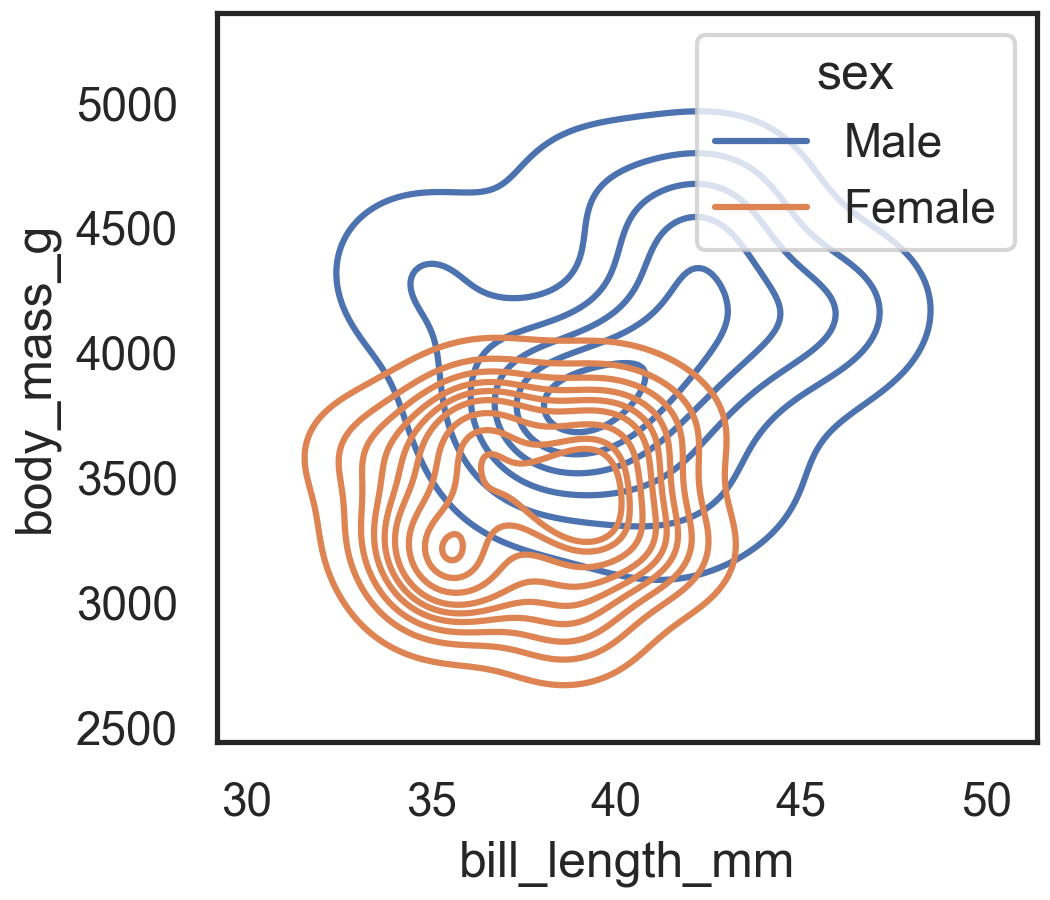
\includegraphics[width=\linewidth]{figures/penguins_distribution.png}
    \caption{Penguins.}
    \label{fig:penguins}
\end{figure}

Nunc id cursus metus aliquam eleifend mi in nulla posuere. Gravida in fermentum et sollicitudin ac orci phasellus. Dolor sit amet consectetur adipiscing elit ut. Commodo viverra maecenas accumsan lacus vel facilisis volutpat. Sem viverra aliquet eget sit amet tellus. Enim nulla aliquet porttitor lacus. Tempor nec feugiat nisl pretium fusce. Diam in arcu cursus euismod quis viverra nibh. Eget egestas purus viverra accumsan in nisl nisi scelerisque eu. Diam sollicitudin tempor id eu nisl nunc. Odio aenean sed adipiscing diam donec adipiscing. Ac tortor vitae purus faucibus ornare suspendisse sed. Vel turpis nunc eget lorem. Gravida cum sociis natoque penatibus et. Nec sagittis aliquam malesuada bibendum arcu vitae elementum curabitur. Porttitor leo a diam sollicitudin. Venenatis tellus in metus vulputate eu scelerisque felis imperdiet. Commodo nulla facilisi nullam vehicula.

\begin{table}
\centering
\caption{Differences in penguins}
\label{tab:features}
\begin{tabular}{lcccccccccc}
\toprule
{} &  count &     max &     min \\
sex    &        &         &         \\
\midrule
Female &   24.0 &  3800.0 &  2900.0 \\
Male   &   23.0 &  4700.0 &  3325.0 \\
\bottomrule
\end{tabular}
\end{table}


Varius quam quisque id diam vel quam. Porta lorem mollis aliquam ut porttitor leo a. Mi in nulla posuere sollicitudin. Diam vel quam elementum pulvinar etiam non. Enim blandit volutpat maecenas volutpat blandit aliquam etiam erat velit. Posuere morbi leo urna molestie. Laoreet suspendisse interdum consectetur libero id faucibus. Tellus orci ac auctor augue mauris augue neque gravida in. Semper auctor neque vitae tempus quam pellentesque nec nam. Diam sit amet nisl suscipit adipiscing. Lectus magna fringilla urna porttitor.

Tincidunt nunc pulvinar sapien et ligula ullamcorper. Adipiscing diam donec adipiscing tristique risus nec feugiat in fermentum. Leo integer malesuada nunc vel risus commodo viverra maecenas accumsan. Bibendum ut tristique et egestas quis ipsum suspendisse ultrices gravida. Consectetur lorem donec massa sapien faucibus et molestie. Nunc sed augue lacus viverra. Tincidunt vitae semper quis lectus nulla at volutpat diam. Nascetur ridiculus mus mauris vitae ultricies. Volutpat commodo sed egestas egestas fringilla phasellus faucibus scelerisque eleifend. Convallis aenean et tortor at risus viverra adipiscing at in. Sagittis id consectetur purus ut faucibus pulvinar elementum integer enim. Convallis posuere morbi leo urna molestie at elementum eu facilisis. Quisque sagittis purus sit amet volutpat consequat mauris. Porta nibh venenatis cras sed.

There are \cite{Tartarini2017PE}




    %! Author = sbbfti
%! Date = 10/06/2020

\section{The Elsevier article class}

\paragraph{Installation} If the document class \emph{elsarticle} is not available on your computer, you can download and install the system package \emph{texlive-publishers} (Linux) or install the \LaTeX\ package \emph{elsarticle} using the package manager of your \TeX\ installation, which is typically \TeX\ Live or Mik\TeX.

\paragraph{Usage} Once the package is properly installed, you can use the document class \emph{elsarticle} to create a manuscript. Please make sure that your manuscript follows the guidelines in the Guide for Authors of the relevant journal. It is not necessary to typeset your manuscript in exactly the same way as an article, unless you are submitting to a camera-ready copy (CRC) journal.

\paragraph{Functionality} The Elsevier article class is based on the standard article class and supports almost all of the functionality of that class. In addition, it features commands and options to format the
\begin{itemize}
\item document style
\item baselineskip
\item front matter
\item keywords and MSC codes
\item theorems, definitions and proofs
\item lables of enumerations
\item citation style and labeling.
\end{itemize}

\section{Front matter}

The author names and affiliations could be formatted in two ways:
\begin{enumerate}[(1)]
\item Group the authors per affiliation.
\item Use footnotes to indicate the affiliations.
\end{enumerate}
See the front matter of this document for examples. You are recommended to conform your choice to the journal you are submitting to.

\section{Bibliography styles}

There are various bibliography styles available. You can select the style of your choice in the preamble of this document. These styles are Elsevier styles based on standard styles like Harvard and Vancouver. Please use Bib\TeX\ to generate your bibliography and include DOIs whenever available.

Here are two sample references: \cite{Feynman1963118,Dirac1953888}.

\bibliography{mybibfile}

\end{document}

\end{document}
